\documentclass[lettersize,journal]{IEEEtran}

\usepackage{amsmath,amssymb,amsfonts}
\usepackage{algorithm}
\usepackage{algorithmic}
\usepackage{array}
\usepackage{booktabs}
\usepackage{multirow}
\usepackage[caption=false,font=footnotesize,labelfont=sf,textfont=sf]{subfig}
\usepackage{textcomp}
\usepackage{stfloats}
\usepackage{url}
\usepackage{graphicx}
\usepackage{cite}
\usepackage[table]{xcolor}
\usepackage{siunitx}
\usepackage[hidelinks]{hyperref}

\setlength{\textfloatsep}{7pt plus 2pt minus 2pt}
\setlength{\dbltextfloatsep}{7pt plus 2pt minus 2pt}
\setlength{\floatsep}{6pt plus 2pt minus 2pt}
\setlength{\abovecaptionskip}{3pt}
\setlength{\belowcaptionskip}{0pt}

\graphicspath{{figures/}}
\hyphenation{op-tical net-works semi-conduc-tor Stein-metz}
\newcommand{\fbar}{\bar{f}}
\newcommand{\Bbar}{\bar{B}}
\newcommand{\Pbar}{\bar{P}_{v}}
\newcommand{\predP}{\widehat{P}_{v}}
\newcommand{\vect}[1]{\boldsymbol{#1}}

\begin{document}

\title{Learnable Symbolic Sparse Identification for Compact and Accurate Magnetic Core-Loss Equations Across Ferrite Materials}

\author{Haoyu Wang,~\IEEEmembership{Graduate Student Member,~IEEE,}
Jialin Zheng,~\IEEEmembership{Member,~IEEE,}
Yihao Wu,~\IEEEmembership{Graduate Student Member,~IEEE,}
Ziyang Xu,~\IEEEmembership{Graduate Student Member,~IEEE,}
and Alex Hanson,~\IEEEmembership{Senior Member,~IEEE}%
\thanks{Haoyu Wang and Alex Hanson are with the Department of Electrical and Computer Engineering, The University of Texas at Austin, Austin, TX 78712 USA.}%
}

\markboth{IEEE Transactions on Power Electronics}%
{Wang \MakeLowercase{\textit{et al.}}: Learnable Symbolic Sparse Identification for Magnetic Core Loss}

\maketitle

\begin{abstract}
Compact magnetic core-loss equations are indispensable for high-frequency magnetic design because they expose scaling trends and can be evaluated inside optimization loops. Existing models, however, force a persistent tradeoff: empirical power laws are transparent but structurally inaccurate over wide operating ranges, whereas machine-learning predictors can be accurate but do not return an equation. This paper proposes a Learnable Symbolic Sparse Identification (LSSI) framework that discovers explicit core-loss equations directly from experimental data. A physics-guided library represents hysteresis, eddy-current, anomalous, saturation, and auxiliary loss behaviors with only ten candidate terms. Unlike fixed-library sparse regression, the fractional exponents and high-frequency roll-off parameters inside these terms are learned jointly with nonnegative sparse coefficients. A hybrid logarithmic and percentage objective equalizes errors across the multi-decade loss range, while staged AdamW optimization, hard projection, contribution pruning, weak raw-coordinate regularization, and support-fixed polishing produce a compact and numerically stable equation. Experimental validation uses 3880 sinusoidal operating points measured at \SI{25}{\degreeCelsius} on Fair-Rite 78, 79, and 95 ferrites by an automated parallel-resonant platform. All three materials identify the same four-term support. Test-set mean absolute percentage errors are \SI{1.93}{\percent}, \SI{0.85}{\percent}, and \SI{1.11}{\percent}, respectively, with $R^2\geq0.9995$. Relative to a 103-term fixed-grid sparse baseline, LSSI reduces the identified equations from 7--11 active terms to four and lowers the three-material mean error from 1.49\% to 1.30\%. A same-split comparison shows that an FNN can further reduce prediction error to 0.40--0.70\%, but it requires 4417 weights and returns no explicit equation. LSSI therefore provides the most accurate compact analytical model in aggregate among the evaluated equation-based approaches, using only 15 learned parameters while remaining directly usable in magnetic design and loss-constrained optimization.
\end{abstract}

\begin{IEEEkeywords}
Core loss, equation discovery, high-frequency magnetics, interpretable machine learning, sparse identification, symbolic regression.
\end{IEEEkeywords}

\section{Introduction}
\IEEEPARstart{T}{he} continuous push toward higher power density has elevated the operating frequencies of magnetic components into the sub-megahertz and megahertz domains \cite{7370781}. Consequently, magnetic core loss increasingly determines converter efficiency, temperature rise, and the minimum feasible magnetic volume. High-fidelity loss modeling over a broad range of frequency $f$ and peak flux density $B$ is nevertheless difficult because the measured volumetric loss $P_v$ is the macroscopic result of several nonlinear mechanisms whose relative importance changes with operating point \cite{1041954}. A model for design must therefore resolve a genuinely two-dimensional nonlinear surface while remaining simple enough to expose the underlying scaling.

Closed-form empirical equations are attractive precisely because they meet the second requirement. The Steinmetz equation (SE), $P_v=k f^{\alpha}B^{\beta}$, directly states the sensitivities to $f$ and $B$ and requires only three parameters \cite{1457110}. Its variants extend the same analytical idea to nonsinusoidal excitation \cite{5955126,10278470}. However, fitting the coefficients of a prescribed structure cannot correct an error in that structure. One power law imposes constant logarithmic slopes, $\partial\ln P_v/\partial\ln f=\alpha$ and $\partial\ln P_v/\partial\ln B=\beta$, across the full operating plane. Real ferrite data exhibit frequency dispersion, flux-dependent exponent drift, and a steep loss upturn near saturation. The SE must average these regimes into one pair of exponents, which preserves simplicity but produces systematic error.

Modern machine-learning (ML) methods remove the prescribed equation and learn the nonlinear map directly. Random forests (RFs), feedforward neural networks (FNNs), transfer-learning models, convolutional networks, and physics-informed neural networks have all demonstrated high prediction accuracy for magnetic materials \cite{10509368,10502151,10232863,10315145,10738458,11126536}. Their flexibility is valuable when temperature, bias, or waveform descriptors enlarge the input space. Yet most such models return a numerical predictor rather than an analytical equation. Thousands of weights or tree nodes do not state which loss mechanism dominates, what fractional exponent has been identified, or how a change in $f$ trades against a change in $B$. Thus, ML improves prediction but does not automatically recover the explicit scaling information that makes the SE useful in magnetic design.

Symbolic regression (SR) attempts to close this gap by discovering a mathematical expression from data \cite{9180100}. Sparse identification is especially compatible with magnetic loss: a library of nonlinear candidate functions is constructed, and a sparse coefficient vector selects only the dominant terms. Recent work has shown the value of this formulation for power-electronic governing equations \cite{11106929,11592694}. In a fixed-library sparse identification (SSI) model, a sufficiently rich library can outperform the SE while preserving a closed form. The difficulty is that the richness must be chosen before training. Magnetic loss is characterized by noninteger exponents, whereas a fixed library samples those exponents on a discrete grid. A coarse grid limits accuracy; a dense grid creates many correlated candidates and represents one physical scaling law by a sum of several neighboring terms. Accuracy is then purchased by losing the sparsity and physical clarity that motivated symbolic identification.

The essential step is therefore to learn not only the coefficients outside the candidate functions, but also the fractional parameters inside them. This paper proposes Learnable Symbolic Sparse Identification (LSSI), in which a compact physics-guided library contains bounded learnable exponents, exponent-drift factors, and high-frequency roll-off parameters. A joint optimization selects the dominant mechanisms and tunes their internal nonlinear parameters simultaneously. In this way, one continuously adaptable term replaces a cluster of fixed-grid terms, while nonnegative coefficients, physical parameter bounds, and explicit pruning preserve a dissipative and readable equation.

Compared with the Letter formulation centered on Fair-Rite 95, the present Regular Paper develops the mathematical connection between fixed-grid and learnable libraries, gives a complete staged optimization and contribution-based support criterion, and evaluates the same framework on three ferrites with distinct operating regions. It also makes the method comparison uniform: SE, RF, FNN, fixed SSI, and LSSI use the same training and test points for every material. This expanded evaluation separates two questions that are often conflated: which model predicts most accurately, and which model provides the most accurate compact equation.

The main contributions are as follows.
\begin{enumerate}
\item A compact, ten-term symbolic library is formulated from magnetic-loss mechanisms. Fractional exponents, flux-dependent exponent drift, and high-frequency roll-off parameters are optimized jointly with nonnegative sparse coefficients.
\item A reproducible staged identification procedure is developed. Normalization, a logarithmic-percentage objective, support pruning, and support-fixed polishing jointly address multi-decade targets, coefficient comparability, and numerical sparsity.
\item The fixed-library sparse method is used as a controlled ablation. Across three ferrites, LSSI reduces 7--11 fixed-grid terms to the same four learnable terms and improves the mean held-out accuracy, directly quantifying the value and the limits of continuous parameter learning.
\item The method is experimentally evaluated on 3880 points covering \SIrange{52.4}{1030}{\kilo\hertz} and approximately \SIrange{4.5}{391}{\milli\tesla}. A common late-stage audit verifies convergence of both sparse coefficients and raw nonlinear coordinates for every material.
\item A uniform comparison against SE, RF, FNN, and SSI quantifies both accuracy and model complexity. A transparent radar-score rubric distinguishes numerical accuracy from compactness, interpretability, design simplicity, and deployment feasibility.
\end{enumerate}

The remainder of the paper is organized as follows. Section~II defines the equation-discovery problem and explains the limitations of fixed symbolic grids. Section~III presents the LSSI library and optimization. Section~IV describes the measurement system and datasets. Sections~V and VI report results and discuss their physical and design implications. Section~VII states the present scope, followed by conclusions in Section~VIII.

\section{Core-Loss Modeling as Equation Discovery}
\subsection{Desired Properties of a Design-Oriented Model}

Let $\mathcal{D}=\{(f_i,B_i,P_{v,i})\}_{i=1}^{N}$ denote measurements under sinusoidal steady-state excitation at a fixed temperature. A useful model should satisfy four requirements. First, it must predict loss accurately throughout the characterized domain rather than only along a single frequency or flux cut. Second, it must remain positive because each retained term represents dissipative behavior. Third, its structure should be compact enough to inspect and embed in optimization. Finally, its parameters should vary continuously so that the model can represent the fractional scaling that is characteristic of ferrite loss.

The SE satisfies compactness and continuity but assumes one mechanism over the entire domain. Black-box regressors satisfy continuity and often accuracy, but not explicit structure. Sparse equation discovery instead writes
\begin{equation}
 \Pbar(\fbar,\Bbar)=\vect{\Theta}(\fbar,\Bbar;\vect{\Lambda})\vect{\Xi},
 \label{eq:general}
\end{equation}
where $\fbar=f/f_{\mathrm{n}}$, $\Bbar=B/B_{\mathrm{n}}$, and $\Pbar=P_v/P_{\mathrm{n}}$ are normalized variables. The library $\vect{\Theta}=[\theta_1,\ldots,\theta_M]$ contains symbolic functions, $\vect{\Xi}=[\xi_1,\ldots,\xi_M]^T\succeq\vect{0}$ contains scaling coefficients, and $\vect{\Lambda}$ collects nonlinear parameters internal to the library. The identified equation is the subset for which $\xi_j>0$ after pruning.

Normalization is not cosmetic. The three physical variables differ by several orders of magnitude, and an unnormalized coefficient threshold would penalize columns according to units rather than physical contribution. Training-set means are used here so that no test information enters the learned scales. The final equation remains dimensional through $f_{\mathrm{n}}$, $B_{\mathrm{n}}$, and $P_{\mathrm{n}}$.

\subsection{Fixed-Grid Sparse Identification and Its Resolution Limit}

The fixed-library sparse identification (SSI) baseline expands $\vect{\Theta}$ with many discrete power-law columns $\fbar^{\alpha}\Bbar^{\beta}$, high-frequency roll-off columns, logarithmic corrections, saturation functions, and low-order auxiliaries. The implementation contains 103 candidates, including $\alpha\in\{1.0,1.2,1.4,1.5,1.6,1.8,2.0,2.2\}$ and $\beta\in\{1.6,1.8,2.0,2.2,2.4,2.5,2.6,2.8,3.0\}$. Each column is normalized before nonnegative AdamW regression and threshold pruning.

This baseline is intentionally expressive and provides an important ablation. Suppose that the data are generated by $\fbar^{1.13}\Bbar^{2.67}$. No column exactly matches this structure. The solver can either select the closest grid point and retain a systematic residual, or combine several correlated columns around the true exponent. Refining the grid reduces approximation error but increases the library size and worsens collinearity. The result is an accuracy--sparsity tradeoff created by the representation rather than by the underlying material. LSSI replaces each cluster of nearby fixed columns with one bounded learnable function.

\subsection{Mathematical Motivation for Learnable Parameters}

The relation between the fixed SSI library and LSSI can be stated directly. Consider a local Steinmetz-type candidate
\begin{equation}
 \theta(\alpha,\beta)=\fbar^{\alpha}\Bbar^{\beta}.
 \label{eq:base_power}
\end{equation}
If the fixed library contains $(\alpha_0,\beta_0)$ but the material follows $(\alpha_0+\Delta\alpha,\beta_0+\Delta\beta)$, then
\begin{align}
 \theta(\alpha_0+\Delta\alpha,\beta_0+\Delta\beta)
 &=\theta(\alpha_0,\beta_0)
 e^{\Delta\alpha\ln\fbar+\Delta\beta\ln\Bbar} \nonumber\\
 &\approx \theta_0+\Delta\alpha\,\theta_0\ln\fbar
 +\Delta\beta\,\theta_0\ln\Bbar,
 \label{eq:taylor_library}
\end{align}
where $\theta_0=\theta(\alpha_0,\beta_0)$. Equation~(\ref{eq:taylor_library}) explains why the fixed SSI baseline requires both neighboring powers and logarithmic correction columns. It is constructing a first-order approximation to a continuously shifted exponent. LSSI instead optimizes $\alpha$ and $\beta$ directly and represents the left-hand side of (\ref{eq:taylor_library}) exactly with one term. The advantage becomes larger when $|\Delta\alpha|$ or $|\Delta\beta|$ is not small, because higher-order fixed-library corrections would otherwise be required.

The same argument gives the nonlinear gradient used during joint training:
\begin{equation}
 \frac{\partial\widehat{\Pbar}}{\partial\alpha_j}
 =\xi_j\theta_j\ln\fbar,\qquad
 \frac{\partial\widehat{\Pbar}}{\partial\beta_j}
 =\xi_j\theta_j\ln\Bbar.
 \label{eq:exponent_gradients}
\end{equation}
Thus, each exponent is informed by how residuals correlate with the logarithmic input coordinates, whereas $\xi_j$ controls the overall magnitude of the corresponding mechanism. For the complete model, the local sensitivity matrix is
\begin{equation}
 \vect{J}=\left[\frac{\partial\widehat{\vect{P}}}{\partial\vect{\Xi}},
 \frac{\partial\widehat{\vect{P}}}{\partial\vect{\Lambda}}\right]
 =\left[\vect{\Theta},\frac{\partial\vect{\Theta}}{\partial\vect{\Lambda}}\vect{\Xi}\right].
 \label{eq:sensitivity_matrix}
\end{equation}
Column scaling and bounded parameterization keep the two blocks numerically comparable. Sparse support is also essential for identifiability: retaining many nearly collinear power-law columns makes $\vect{J}^{T}\vect{J}$ ill-conditioned and allows several coefficient combinations to describe the same local surface. Pruning reduces this redundancy before the final nonlinear polishing step.

\section{Learnable Symbolic Sparse Identification}
\subsection{Physics-Guided Learnable Library}

Fig.~\ref{fig:framework} summarizes the LSSI workflow. The raw dataset is normalized, the full library is evaluated, sparse coefficients and internal parameters are jointly updated, weak candidates are removed, and the surviving support is polished to form the explicit equation.

\begin{figure*}[t]
 \centering
 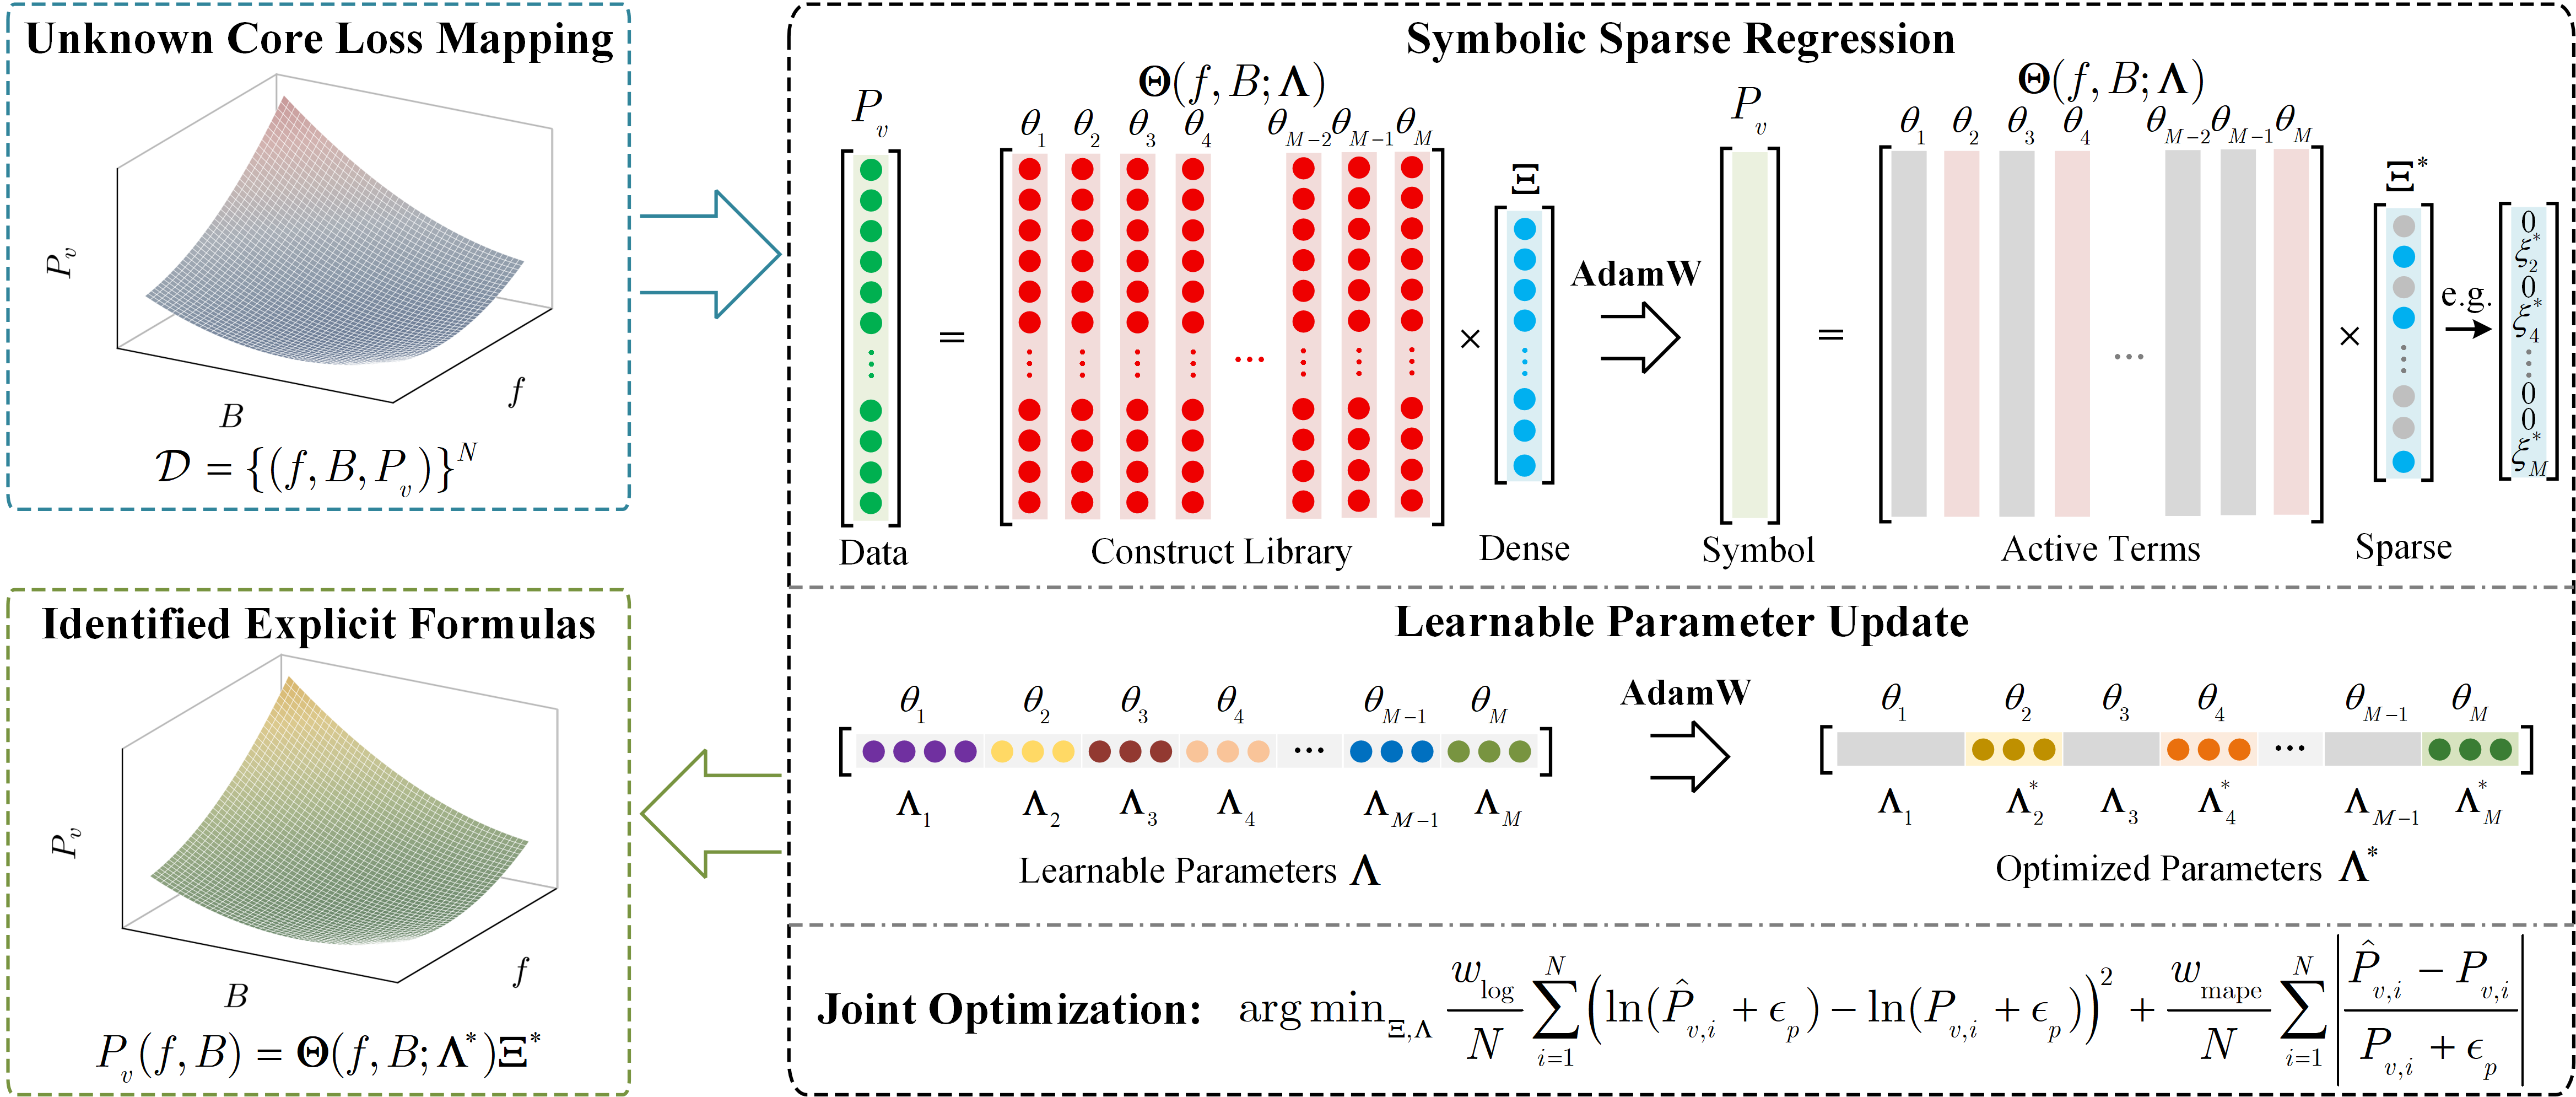
\includegraphics[width=0.88\textwidth]{Figure1_framework.png}
 \caption{Proposed LSSI workflow. A compact physics-guided candidate library is evaluated on normalized measurements. Sparse nonnegative coefficients select the active mechanisms while bounded internal parameters adapt their fractional scaling and high-frequency behavior. The schematic shows the data-fit component; (\ref{eq:loss}) gives the complete objective including raw-coordinate regularization.}
 \label{fig:framework}
\end{figure*}

The ten candidates are listed in Table~\ref{tab:library}. Two differentiable roll-off factors are defined as
\begin{equation}
 R_h(\fbar)=\frac{1}{1+(\fbar/\bar f_{c,h})^{p_h}},\qquad
 R_e(\fbar)=\frac{1}{1+(\fbar/\bar f_{c,e})^{p_e}}.
 \label{eq:rolloff}
\end{equation}
The explicit $h$ and $e$ subscripts prevent ambiguity between the two learned cutoffs. The apparent hysteresis flux exponent is allowed to drift with flux density,
\begin{equation}
 \beta_h'(\Bbar)=\beta_h+\gamma_h\ln(\Bbar+\epsilon),
 \label{eq:drift}
\end{equation}
which is equivalent to a smooth quadratic dependence on $\ln\Bbar$ in logarithmic coordinates. This compactly represents curvature that would otherwise require multiple fixed exponents.

\begin{table*}[t]
\centering
\caption{Physics-Guided Candidate Library Used for All Three Materials}
\label{tab:library}
\renewcommand{\arraystretch}{1.15}
\begin{tabular}{ccll}
\toprule
Index & Candidate $\theta_j(\fbar,\Bbar)$ & Intended behavior & Learnable internal parameters \\
\midrule
1 & $\fbar^{\alpha_h}\Bbar^{\beta_h+\gamma_h\ln(\Bbar+\epsilon)}R_h(\fbar)$ & Hysteresis-like loss with exponent drift and dispersion & $\alpha_h,\beta_h,\gamma_h,\bar f_{c,h},p_h$ \\
2 & $\fbar^{\alpha_e}\Bbar^{\beta_e}R_e(\fbar)$ & Classical eddy-current-like loss with dispersion & $\alpha_e,\beta_e,\bar f_{c,e},p_e$ \\
3 & $\fbar^{\alpha_a}\Bbar^{\beta_a}R_e(\fbar)$ & Anomalous/excess contribution & $\alpha_a,\beta_a$ \\
4 & $\fbar^{\alpha_s}\Bbar^{\beta_s}$ & Unconstrained high-flux power-law correction & $\alpha_s,\beta_s$ \\
5 & $\fbar\exp(\delta\Bbar)$ & Exponential high-flux candidate & $\delta$ \\
6--7 & $\fbar\Bbar$, $\fbar\Bbar^2$ & Low-order cross-coupling corrections & none \\
8--10 & $\fbar$, $\Bbar$, $1$ & Isolated drift and offset corrections & none \\
\bottomrule
\end{tabular}
\end{table*}

Candidates 1--3 are inspired by the conventional decomposition of magnetic loss into hysteresis, classical eddy-current, and anomalous contributions \cite{1041954}. Their labels are interpretive rather than a claim of microscopic separation: parameters are learned from macroscopic data, so a retained term can aggregate more than one process with similar scaling. Candidate 4 captures a steep high-flux contribution without forcing a predetermined saturation exponent. Candidate 5 offers a distinct exponential alternative. Candidates 6--10 protect the principal terms from absorbing small offsets or low-order trends. Sparsification determines which of these functions are needed for a particular material.

\subsection{Bounded Parameterization and Thermodynamic Consistency}

Each learned exponent is constrained to a physically plausible interval. Direct clipping after every gradient step can stall a parameter at a boundary. LSSI instead optimizes an unconstrained raw variable $z$ and maps it smoothly to $[\lambda_{\min},\lambda_{\max}]$:
\begin{equation}
 \lambda=\lambda_{\min}+(\lambda_{\max}-\lambda_{\min})\operatorname{sigmoid}(z).
 \label{eq:sigmoid}
\end{equation}
The coefficient vector is projected onto the nonnegative orthant after each update. Consequently, every active candidate contributes nonnegative loss within the characterized domain, and the complete prediction cannot become negative through cancellation. This constraint also improves interpretability: sparsity is not manufactured by subtracting two large, nearly identical terms.

The bounds in Table~\ref{tab:hyper} are shared by all materials. Hysteresis-like frequency scaling is centered near unity, classical eddy scaling near two, anomalous scaling near $1.5$, and the saturation correction is allowed a steeper flux exponent. The roll-off cutoffs are expressed in units of $f_{\mathrm{n}}$, which makes the same bounds applicable to materials with different useful frequency regions.

\subsection{Multi-Scale Objective}

The measured losses span more than two orders of magnitude. An ordinary mean-squared error in physical units would prioritize the largest-loss samples, while a pure percentage loss can be sensitive to the smallest target. The adopted objective combines logarithmic squared error and mean absolute percentage error (MAPE):
\begin{align}
 \mathcal{L}(\vect{\Xi},\vect{z})={}&\frac{w_{\log}}{N}\sum_{i=1}^{N}
 \left[\ln(\widehat{\bar P}_{v,i}+\epsilon)-\ln(\bar P_{v,i}+\epsilon)\right]^2 \nonumber\\
 &+\frac{w_{\mathrm{p}}}{N}\sum_{i=1}^{N}
 \left|\frac{\widehat{\bar P}_{v,i}-\bar P_{v,i}}{\bar P_{v,i}+\epsilon}\right|
 +\frac{\lambda_z}{L}\lVert\vect{z}\rVert_2^2.
 \label{eq:loss}
\end{align}
Equal weights $w_{\log}=w_{\mathrm{p}}=0.5$ and $\lambda_z=2.5\times10^{-4}$ are used throughout, where $L$ is the number of raw nonlinear coordinates. The logarithmic term penalizes multiplicative mismatch symmetrically across the range, while the MAPE term aligns training with the primary reported metric. The final term does not sparsify the equation; it selects a finite, reproducible representative when different coefficient--parameter combinations generate nearly indistinguishable library columns over the finite measurement domain. No material-specific weight is introduced.

\subsection{Staged Sparse Optimization}

The optimization has four stages, given in Algorithm~\ref{alg:lssi}. First, only $\vect{\Xi}$ is updated during a warm-up period. This allows all columns to establish comparable scales before the nonlinear functions move. Second, $\vect{\Xi}$ and $\vect{\Lambda}$ are jointly updated with AdamW. AdamW decay is applied only to $\vect{\Xi}$, whereas the explicit and much weaker $\lambda_z$ term regularizes the raw coordinates. This distinction is important: coefficient decay promotes structural competition, while raw-coordinate regularization resolves flat parameter tradeoffs without deciding support. Third, a ramped threshold removes coefficients that remain weak late in training. The delayed schedule avoids eliminating a term before its internal exponents reach a useful region. Fourth, once the support is fixed, limited-memory BFGS (L-BFGS) polishing removes coefficient shrinkage bias while retaining the weak coordinate regularizer. A final mean-contribution threshold of $0.1\%$ eliminates numerically nonzero candidates whose library columns have collapsed during parameter adaptation, followed by one support-fixed refit.

\begin{algorithm}[t]
\caption{Learnable Symbolic Sparse Identification}
\label{alg:lssi}
\begin{algorithmic}[1]
\STATE Normalize training data by $f_{\mathrm{n}}$, $B_{\mathrm{n}}$, $P_{\mathrm{n}}$.
\STATE Initialize $\vect{\Xi}\geq0$, raw parameters $\vect{z}$, and support mask $\vect{d}=\vect{1}$.
\STATE Warm up $\vect{\Xi}$ with $\vect{z}$ frozen.
\FOR{each joint-discovery epoch}
  \STATE Map $\vect{z}$ to bounded $\vect{\Lambda}$ using (\ref{eq:sigmoid}).
  \STATE Update $\vect{\Xi}$ and $\vect{z}$ using gradients of (\ref{eq:loss}).
  \STATE Project $\vect{\Xi}\leftarrow\max(\vect{0},\vect{\Xi})\odot\vect{d}$.
  \STATE After the pruning start, ramp $\tau$ and set $d_j=0$ when $\xi_j<\tau$.
\ENDFOR
\STATE Freeze the support and jointly polish surviving parameters with L-BFGS.
\STATE Remove terms contributing less than $0.1\%$ and refit once.
\RETURN Explicit equation, parameters, support, and validation metrics.
\end{algorithmic}
\end{algorithm}

The AdamW moment equations follow their standard form. With gradient $\vect{g}_t=\nabla\mathcal{L}$, bias-corrected moments $\widehat{\vect{m}}_t$ and $\widehat{\vect{v}}_t$, learning rate $\eta$, and coefficient decay $\lambda_{\mathrm{wd}}$, the two parameter blocks are updated by
\begin{align}
 \vect{\Xi}_{t+1}&=\Pi_{\mathbb{R}_+^M}\!\left[\vect{\Xi}_t-\eta\left(
 \frac{\widehat{\vect{m}}^{\Xi}_t}{\sqrt{\widehat{\vect{v}}^{\Xi}_t}+\epsilon_a}
 +\lambda_{\mathrm{wd}}\vect{\Xi}_t\right)\right], \label{eq:update_xi}\\
 \vect{z}_{t+1}&=\vect{z}_t-\eta
 \frac{\widehat{\vect{m}}^{z}_t}{\sqrt{\widehat{\vect{v}}^{z}_t}+\epsilon_a},\quad
 \vect{g}^{z}_t=\nabla_{\vect z}\mathcal{L}. \label{eq:update_z}
\end{align}
The binary mask makes pruning irreversible within one run. This converts the continuous optimization into an explicit model-selection path and prevents eliminated terms from reappearing due to optimizer momentum.

\begin{table}[t]
\centering
\caption{Shared LSSI Hyperparameters and Bounds}
\label{tab:hyper}
\renewcommand{\arraystretch}{1.08}
\begin{tabular}{lc@{\qquad}lc}
\toprule
Quantity & Value & Quantity & Value \\
\midrule
Warm-up epochs & 1200 & Joint epochs & 40000 \\
Learning rate & 0.001 & Weight decay & 0.002 \\
$w_{\log},w_{\mathrm{p}}$ & 0.5, 0.5 & $\lambda_z$ & $2.5\times10^{-4}$ \\
Prune start & 75\% & Max. threshold & 0.001 \\
$\alpha_h$ & [0.8,1.3] & $\beta_h$ & [2.0,2.8] \\
$\alpha_e,\beta_e$ & [1.8,2.2] & $\alpha_a,\beta_a$ & [1.3,1.7] \\
$\alpha_s$ & [0.9,1.2] & $\beta_s$ & [2.8,3.5] \\
$\bar f_{c,e}$ & [2,6] & $\bar f_{c,h}$ & [3,10] \\
$p_e,p_h$ & [1,4] & Final contribution & 0.1\% \\
\bottomrule
\end{tabular}
\end{table}

\section{Experimental Platform and Datasets}
\subsection{Automated Parallel-Resonant Characterization}

The identification data were obtained using the automated parallel-resonant measurement platform reported in \cite{11121265}. The hardware integrates two digitally configurable capacitor sequences, high-frequency analog conditioning, a direct-digital-synthesis source, and a TMS320F28379D-based control subsystem. The local controller selects the resonant and blocking capacitors, synthesizes the drive and orthogonal reference signals, digitizes isolated dc outputs from the conditioning channels, and advances frequency and amplitude sweeps without oscilloscope-based postprocessing.

Each capacitor sequence contains ten independently switched branches, supporting a large set of resonant configurations. Electromechanical relays are used in the present sub-megahertz implementation; parallel relays reduce effective on-resistance in large-capacitance branches. The device under test is placed between the two sequences to reduce interconnect parasitics. Four- or five-turn windings keep winding loss small relative to the measured core loss. Independent comparisons against manufacturer data showed that most points fall within approximately $\pm5\%$, with a maximum discrepancy below $13\%$ over the evaluated materials \cite{11121265}. The system acquired 1320 points in a representative sweep in about \SI{20}{\second}, making dense two-dimensional datasets practical.

Fig.~\ref{fig:hardware} shows the integrated characterization board. The resonant capacitor banks and the device under test occupy the lower half of the board, while the isolated conditioning circuits, power-amplifier interface, and DSP controller are placed close to their associated signal paths. This compact arrangement reduces the wiring-dependent parasitics that otherwise become significant near \SI{1}{\mega\hertz}.

\begin{figure}[t]
 \centering
 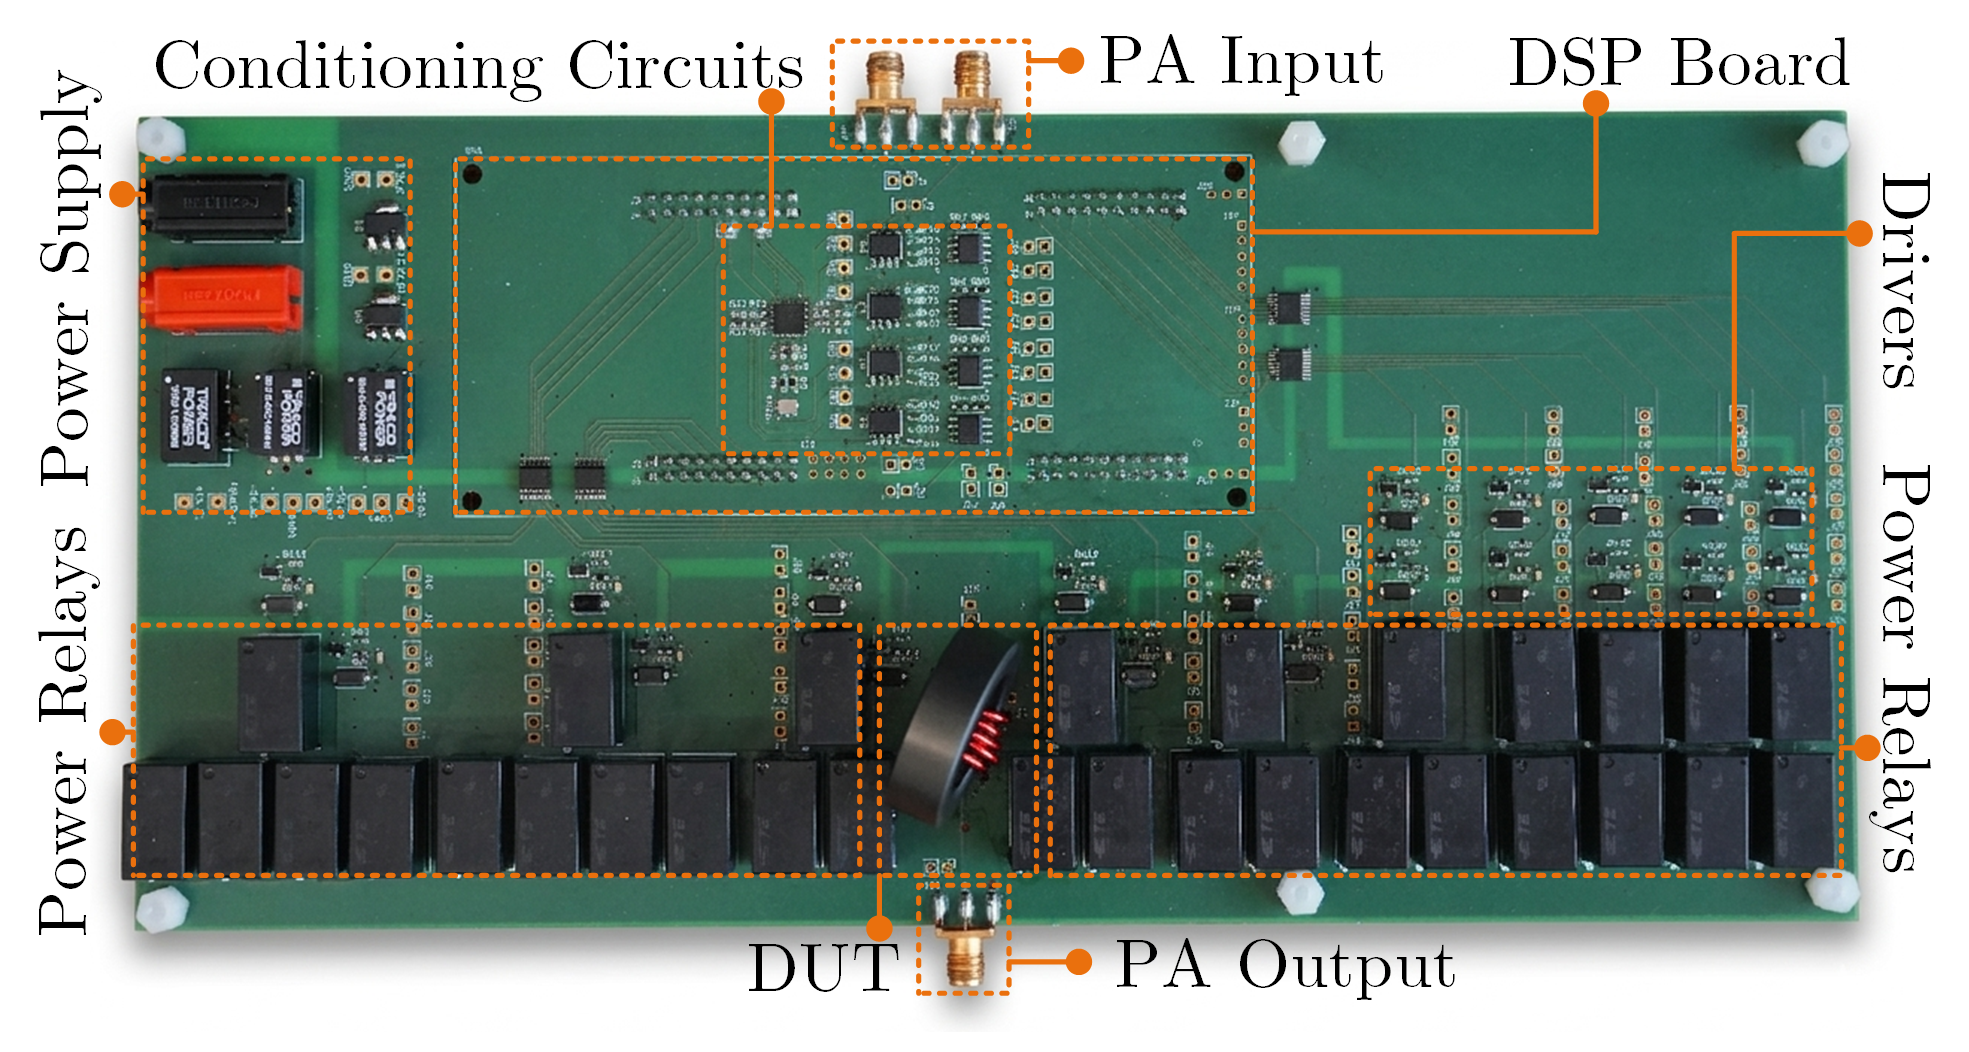
\includegraphics[width=\columnwidth]{Figure4_measurement_hardware.png}
 \caption{Automated parallel-resonant core-loss characterization hardware used to acquire the three material datasets. The two switched capacitor sequences surround the device under test; the DSP board controls the relays, drive signals, and data acquisition.}
 \label{fig:hardware}
\end{figure}

Before equation identification, the acquisition chain was checked against Fair-Rite datasheet curves \cite{11121265}. The measured trajectories reproduce the manufacturer trends over the available frequency lines, reducing the risk that frequency-dependent acquisition bias is interpreted as an additional loss mechanism.

The measurement platform is not part of the LSSI training loop, but it is essential to the validity of equation discovery. Sparse regression cannot distinguish physical curvature from systematic acquisition error unless the source data have high signal fidelity. Automated switching also produces a consistent sampling procedure across materials, so differences in identified parameters can be interpreted as material behavior rather than operator-dependent test variation.

\subsection{Materials, Coverage, and Data Split}

Three manganese-zinc ferrites are evaluated: Fair-Rite 78, 79, and 95. Their measured ranges and normalization constants are summarized in Table~\ref{tab:data}. The combined dataset contains 3880 positive operating points at \SI{25}{\degreeCelsius}. FR78 emphasizes lower-loss behavior and extends to \SI{1030}{\kilo\hertz}; FR79 includes the largest observed loss and flux density; FR95 is the material used for the detailed method comparison. Together they exercise the same candidate library under substantially different loss surfaces.

\begin{table*}[t]
\centering
\caption{Experimental Datasets and Training-Mean Normalization}
\label{tab:data}
\renewcommand{\arraystretch}{1.12}
\begin{tabular}{lcccccccc}
\toprule
Material & Samples & Train/Test & $f$ (kHz) & $B$ (mT) & $P_v$ (mW/cm$^3$) & $f_{\mathrm{n}}$ (kHz) & $B_{\mathrm{n}}$ (mT) & $P_{\mathrm{n}}$ (mW/cm$^3$) \\
\midrule
FR78 & 1320 & 1056/264 & 53.4--1030 & 4.52--189.92 & 1.37--374.24 & 382.79 & 44.71 & 59.80 \\
FR79 & 1240 & 992/248  & 59.5--893.1 & 12.53--378.00 & 7.76--2004.31 & 360.32 & 88.45 & 288.66 \\
FR95 & 1320 & 1056/264 & 52.4--1029 & 10.97--391.09 & 7.16--1643.80 & 372.57 & 102.60 & 303.95 \\
\bottomrule
\end{tabular}
\end{table*}

Points are sorted lexicographically by frequency and flux density. Every fifth point is assigned to the test set, and the remaining 80\% form the training set. This deterministic interleaved split distributes held-out points across the operating domain and is applied identically to SE, SSI, and LSSI. It primarily tests interpolation within the measured envelope; extrapolation outside that envelope is addressed separately in Section~VII. All reported error statistics are calculated in physical units after undoing normalization.

\section{Identification Results}
\subsection{Identified Common Equation}

All three materials converge to the same support, $\{\theta_1,\theta_2,\theta_4,\theta_9\}$. The resulting common-form equation is
\begin{align}
 \Pbar={}&\xi_1\fbar^{\alpha_h}
 \Bbar^{\beta_h+\gamma_h\ln(\Bbar+\epsilon)}R_h(\fbar)
 +\xi_2\fbar^{\alpha_e}\Bbar^{\beta_e}R_e(\fbar) \nonumber\\
 &+\xi_4\fbar^{\alpha_s}\Bbar^{\beta_s}+\xi_9\Bbar.
 \label{eq:identified}
\end{align}
The material dependence is contained in continuous parameters rather than in a different hand-selected topology. Table~\ref{tab:identified} lists the learned values. The notation $f_{c,h}$ and $f_{c,e}$ is used explicitly because both terms contain a roll-off factor; this avoids the ambiguous numbered cutoffs that can otherwise be inadvertently interchanged.

\begin{table*}[t]
\centering
\caption{Identified Four-Term LSSI Parameters}
\label{tab:identified}
\renewcommand{\arraystretch}{1.1}
\resizebox{\textwidth}{!}{%
\begin{tabular}{lrrrrrrrrrrrrrrr}
\toprule
Material & $\xi_1$ & $\xi_2$ & $\xi_4$ & $\xi_9$ & $\alpha_h$ & $\beta_h$ & $\gamma_h$ & $\alpha_e$ & $\beta_e$ & $\alpha_s$ & $\beta_s$ & $f_{c,h}$ (kHz) & $p_h$ & $f_{c,e}$ (kHz) & $p_e$ \\
\midrule
FR78 & 0.6191 & 0.7402 & 0.2711 & 0.0267 & 1.107 & 2.755 & $-0.537$ & 2.188 & 2.050 & 1.179 & 3.194 & 2903 & 2.947 & 1707 & 3.816 \\
FR79 & 0.6536 & 0.2007 & 0.5440 & 0.0168 & 1.161 & 2.101 & $-0.360$ & 2.060 & 2.093 & 1.124 & 3.073 & 2661 & 2.943 & 1540 & 3.114 \\
FR95 & 0.6627 & 0.8623 & 0.2371 & 0.0171 & 1.163 & 2.685 & $-0.387$ & 2.184 & 1.993 & 1.161 & 3.200 & 1830 & 1.472 & 1176 & 3.908 \\
\bottomrule
\end{tabular}%
}
\end{table*}

The FR95 values align with the expected scaling of the first two physical blocks: the hysteresis-like frequency exponent is $1.163$, while the eddy-current-like exponents are $\alpha_e=2.184$ and $\beta_e=1.993$. The saturation correction has a substantially larger flux exponent, $\beta_s=3.200$. Importantly, these values are not selected from a grid; they are the continuous solution of the joint optimization.

\subsection{Cross-Material Held-Out Accuracy}

The three-material results follow the same evidence chain as the detailed Letter study: predicted-versus-measured agreement establishes accuracy; train/test residual distributions test bias and overfitting; and residual trends versus $B$ and $f$ test whether a systematic physical dependence remains unmodeled. Every diagnostic is presented as one row ordered FR78, FR79, and FR95, so that the same visual test is applied to all materials. Table~\ref{tab:data} shows that the frequency ranges are similar but the accessible flux-density and loss ranges differ substantially: FR78 occupies the lowest-loss region, FR79 reaches the largest $P_v$, and FR95 spans a broad high-flux/high-frequency domain. Thus, the common structure is tested on three distinct nonlinear surfaces rather than replicated datasets.

Fig.~\ref{fig:validation} compares held-out predictions with measurements. FR78 achieves a MAPE of $1.93\%$ and $R^2=0.9997$; FR79 achieves $0.85\%$ and $R^2=0.9995$; FR95 achieves $1.11\%$ and $R^2=0.9999$. The corresponding RMSE values are 1.17, 7.65, and \SI{3.52}{\milli\watt\per\cubic\centi\meter}. RMSE is larger for FR79 because its measured losses reach \SI{2004}{\milli\watt\per\cubic\centi\meter}; its percentage error is nevertheless the smallest. The logarithmic parity axes confirm that agreement is not limited to the high-loss samples.

\begin{figure*}[t]
 \centering
 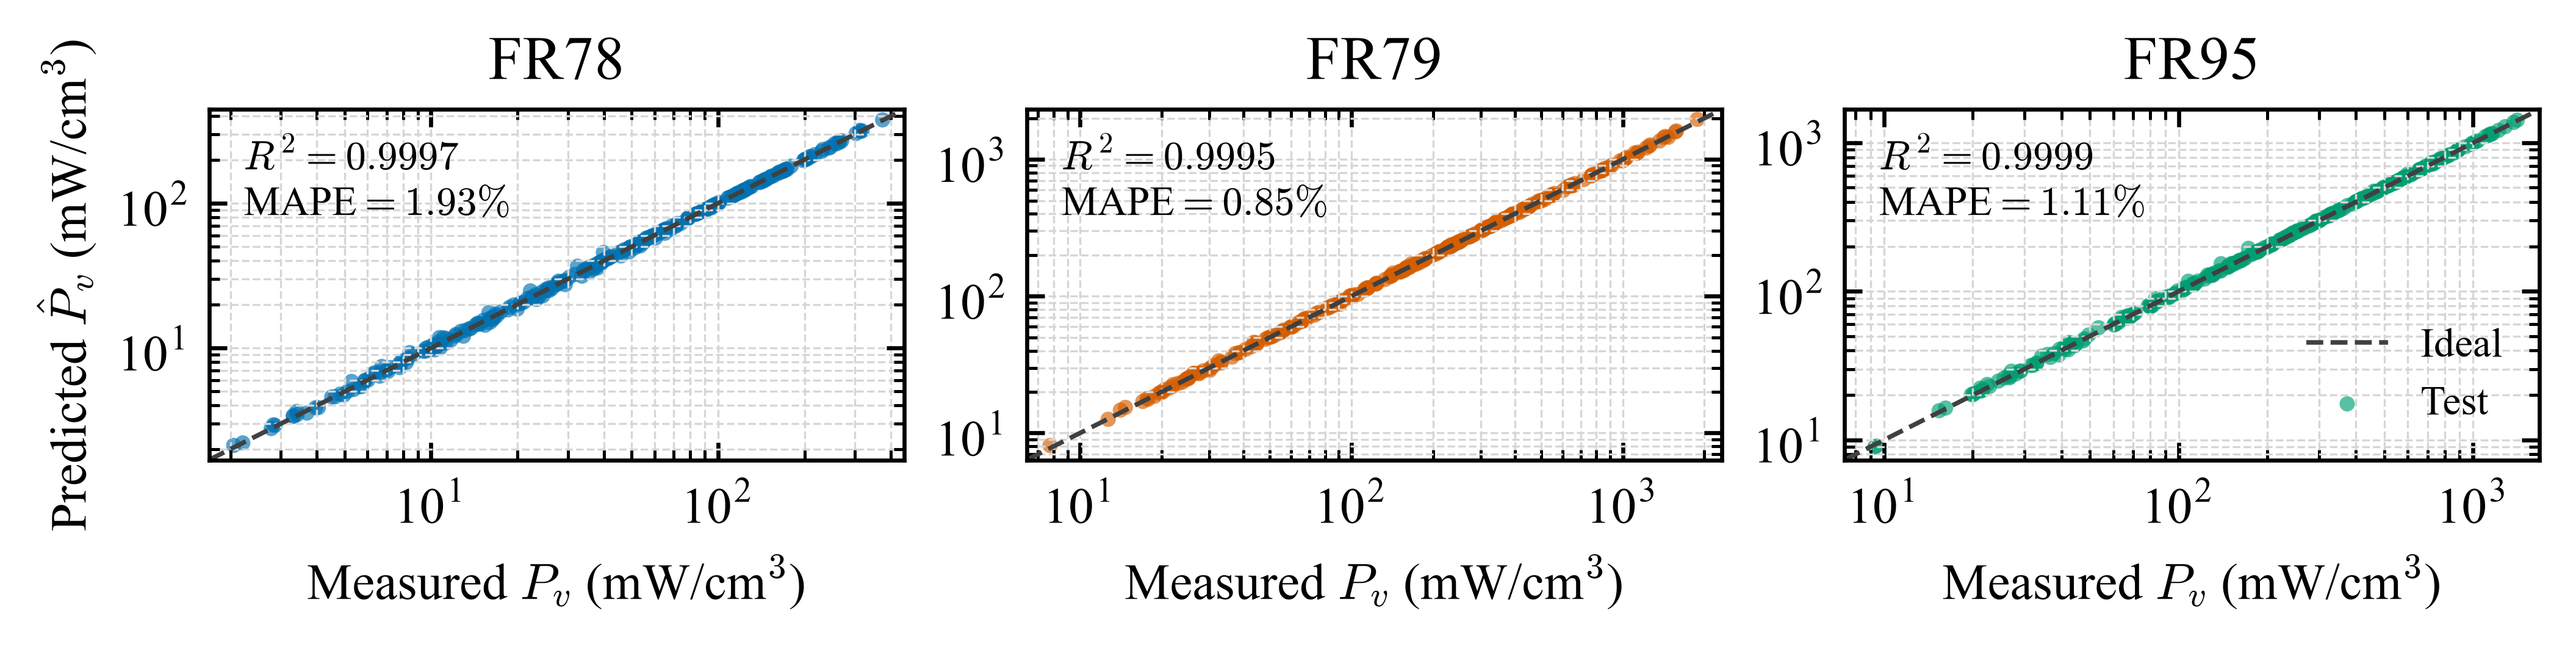
\includegraphics[width=0.98\textwidth]{Figure7_lssi_validation.png}
 \caption{Held-out LSSI predictions versus measurements. From left to right: FR78, FR79, and FR95. The dashed line is the ideal relation.}
 \label{fig:validation}
\end{figure*}

The residual histograms in Fig.~\ref{fig:residual_histograms} are concentrated about zero for both splits. The train/test means are $-0.086/-0.093\%$, $0.101/0.082\%$, and $0.276/0.348\%$ for FR78, FR79, and FR95, respectively. Their corresponding standard deviations are $3.16/3.14\%$, $1.35/1.28\%$, and $1.96/1.93\%$. The nearly identical train and test distributions indicate that the four-term equations generalize to interleaved held-out operating points rather than memorizing the training set. FR78 has the widest percentage distribution because its data extend to the smallest absolute loss, where a small absolute deviation produces a larger relative error.

\begin{figure*}[t]
 \centering
 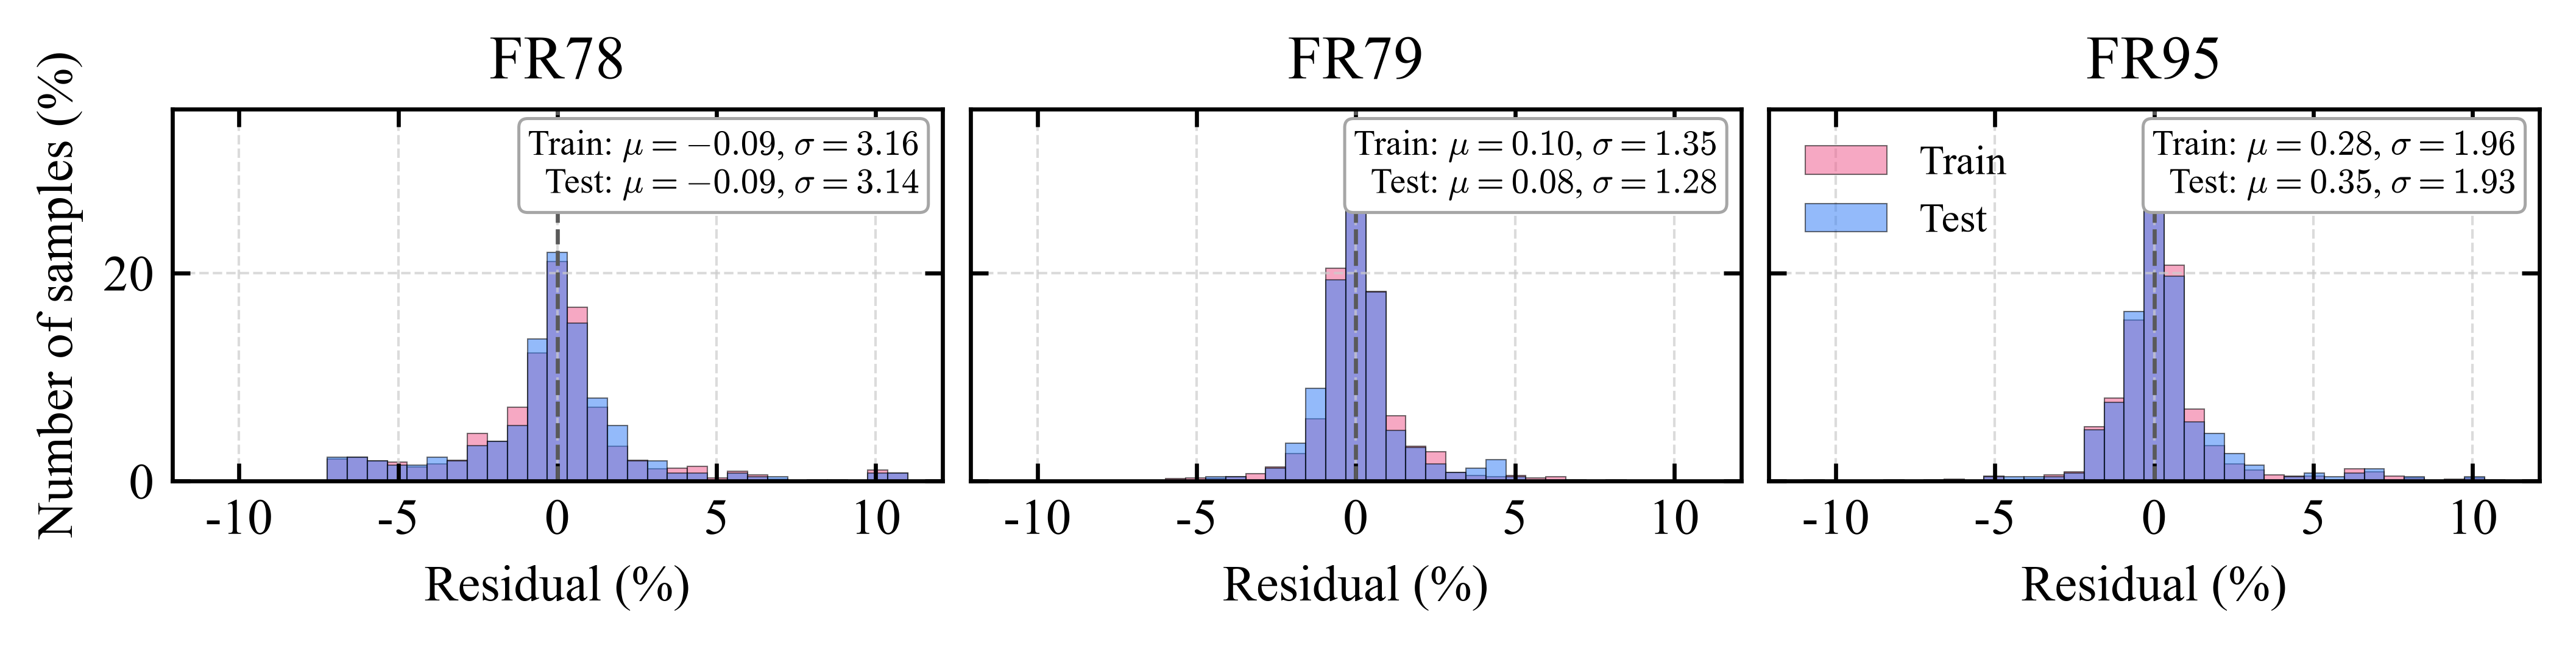
\includegraphics[width=0.98\textwidth]{Figure8_residual_histograms.png}
 \caption{Training and held-out LSSI residual distributions. From left to right: FR78, FR79, and FR95. Each histogram is normalized by its split size so the 80/20 sample counts can be compared directly.}
 \label{fig:residual_histograms}
\end{figure*}

Fig.~\ref{fig:residual_flux} resolves the same residuals along flux density. All three materials show the Letter's characteristic heteroscedastic pattern: the largest percentage excursions occur at the smallest $B$, where measured loss and measurement signal are smallest, and the residual envelope contracts toward the interior of the domain. FR79 has the narrowest envelope, consistent with its $0.85\%$ test MAPE. At larger $B$, none of the materials exhibits a persistent positive or negative band. The model therefore captures the high-flux curvature with the learned $\theta_4$ term rather than leaving a monotonic saturation-related residual.

\begin{figure*}[t]
 \centering
 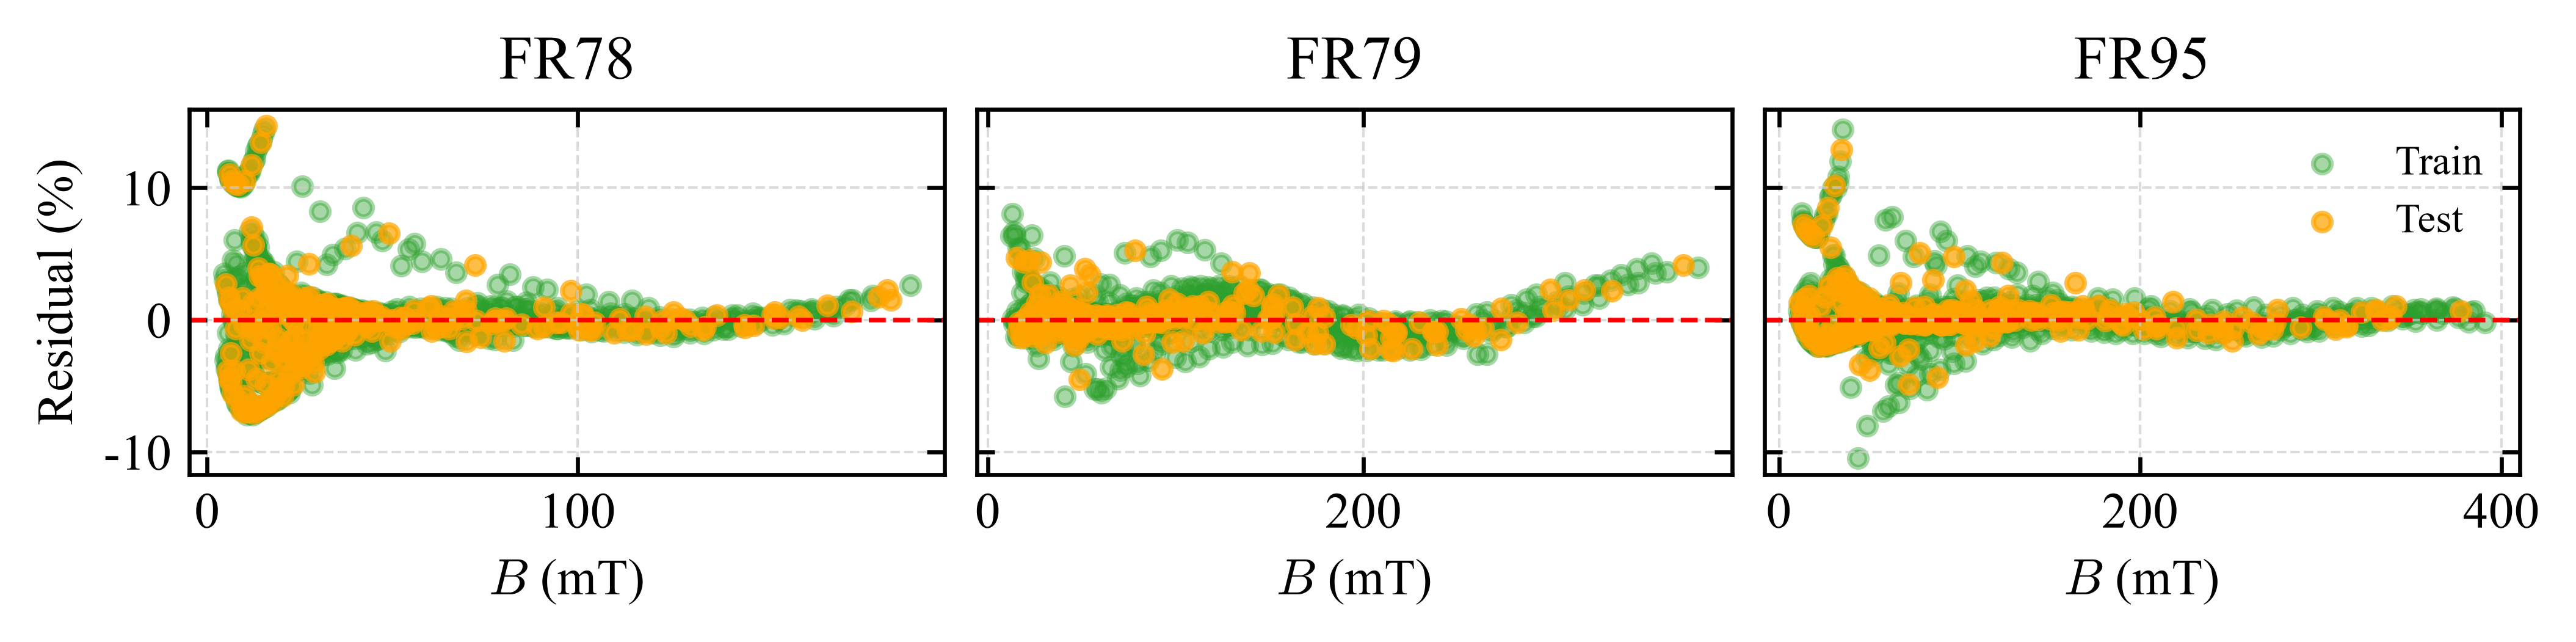
\includegraphics[width=0.98\textwidth]{Figure9_residual_vs_flux.png}
 \caption{Training and held-out percentage residuals versus flux-density amplitude. From left to right: FR78, FR79, and FR95.}
 \label{fig:residual_flux}
\end{figure*}

Fig.~\ref{fig:residual_frequency} tests the complementary frequency coordinate. Small bands appear because measurements were acquired at discrete frequency settings, but the test points follow the same bands as the training points. The low-frequency and near-\SI{1}{\mega\hertz} edge excursions are reproduced across FR78 and FR95 without a steadily increasing error through the interior. FR79 remains within a visibly tighter band across its measured frequency range. Most importantly, no material exhibits a one-sided residual drift over the complete $f$ axis. Together with Fig.~\ref{fig:residual_flux}, this rejects the hypothesis that the low MAPE is obtained by averaging an omitted frequency- or flux-dependent mechanism.

\begin{figure*}[t]
 \centering
 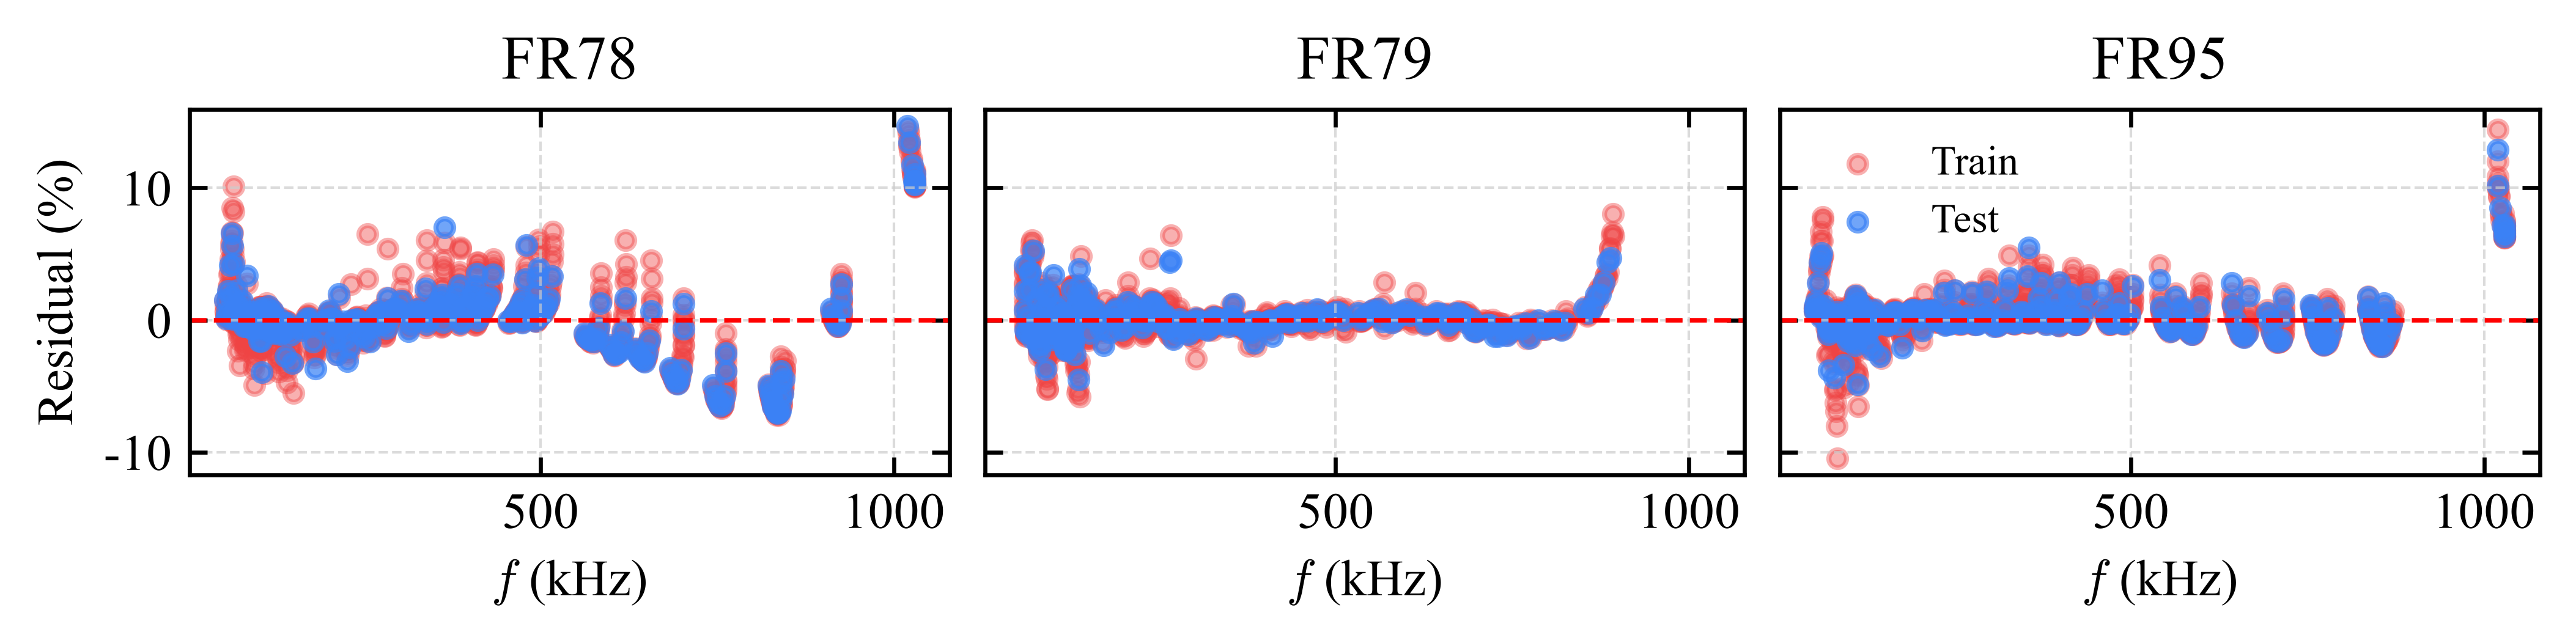
\includegraphics[width=0.98\textwidth]{Figure10_residual_vs_frequency.png}
 \caption{Training and held-out percentage residuals versus frequency. From left to right: FR78, FR79, and FR95.}
 \label{fig:residual_frequency}
\end{figure*}

The near-equality of training and test errors provides the final generalization check. Train/test MAPE pairs are $1.97/1.93\%$ for FR78, $0.85/0.85\%$ for FR79, and $1.13/1.11\%$ for FR95. Test performance is not obtained by using material-specific libraries, bounds, penalties, or thresholds: only the learned parameter values change. The four diagnostics therefore establish a common experimental conclusion: LSSI remains nearly unbiased on unseen points, the residual width does not grow from training to testing, and no systematic trend persists along either physical input.

\subsection{Training Evolution and Support Formation}

The prediction-space diagnostics establish final-equation quality; the optimization trajectories show how the common structure forms. Fig.~\ref{fig:coefficient_evolution} tracks all ten entries of $\vect{\Xi}$ through coefficient-only warm-up, joint discovery, and terminal polishing. During the first 1200 epochs, the nonlinear coordinates are frozen while the candidate coefficients establish comparable scales. After the dotted boundary, $\vect{\Xi}$ and $\vect{\Lambda}$ are jointly optimized. For every material, the same four coefficients remain nonzero while the other six collapse, providing process-level evidence for support $\{\theta_1,\theta_2,\theta_4,\theta_9\}$.

\begin{figure*}[t]
 \centering
 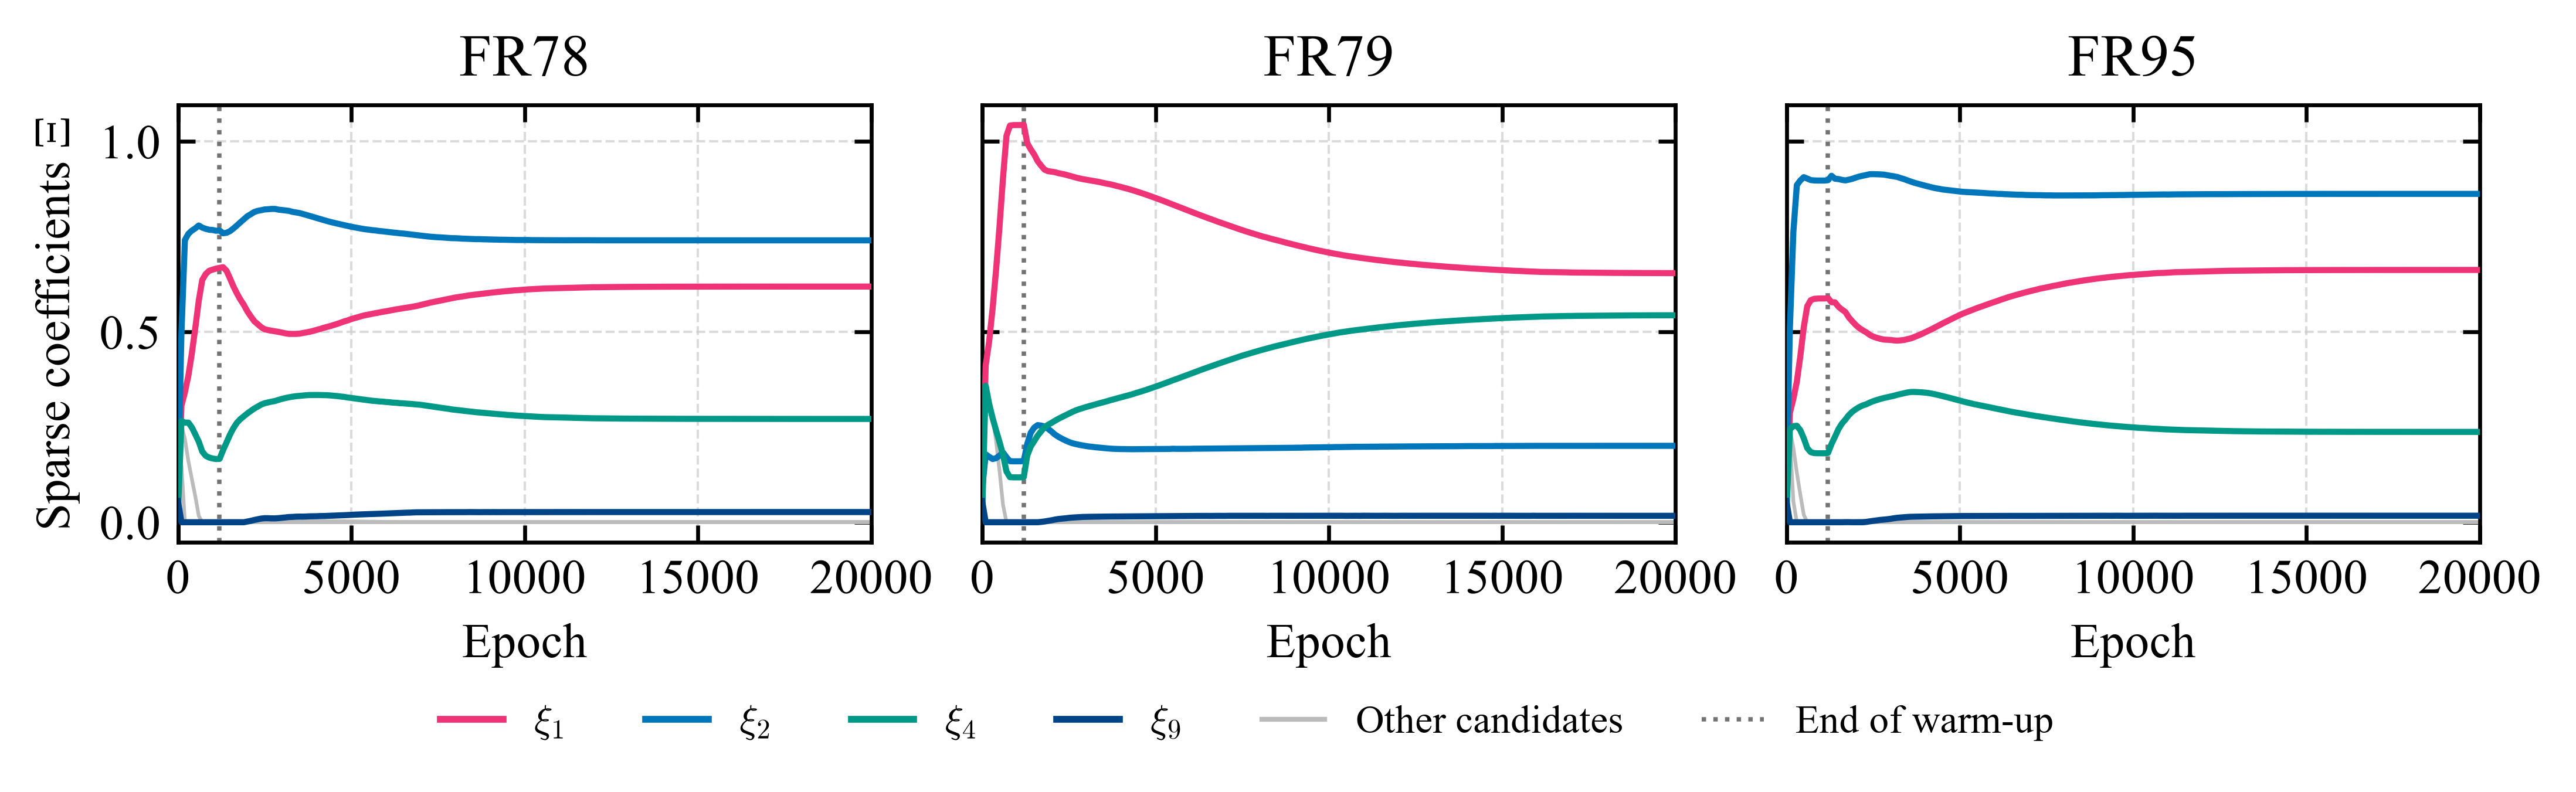
\includegraphics[width=0.98\textwidth]{Figure_parameter_evolution_coefficients.png}
\caption{Evolution of the ten sparse coefficients during LSSI training. From left to right: FR78, FR79, and FR95. Colored curves denote the common retained support; gray curves denote the six candidates that are ultimately pruned. The dotted line marks the end of coefficient-only warm-up. For clarity, only the first 20,000 epochs are displayed.}
 \label{fig:coefficient_evolution}
\end{figure*}

The paths remain material-specific. For FR78 and FR95, $\xi_2$ rapidly becomes largest while $\xi_1$ redistributes after warm-up. For FR79, $\xi_1$ and $\xi_4$ exchange weight before settling, consistent with its final $54.8\%$ saturation-term contribution. The small $\xi_9$ correction approaches a nonzero value for every material. Thus, common topology emerges under different learned balances rather than from forced coefficient equality.

Fig.~\ref{fig:parameter_evolution} shows the eleven raw optimizer coordinates of the retained functions. They remain fixed during warm-up and move continuously after joint discovery starts, as prescribed by Algorithm~1. Without a coordinate preference, FR79 exhibits a shallow compensation direction in which the hysteresis-like and saturation terms exchange amplitude while producing almost the same total surface. The weak $\ell_2$ term selects a finite raw-coordinate neighborhood along this data-equivalent valley. From (\ref{eq:sigmoid}), the map sensitivity is
\begin{equation}
 \frac{\partial\lambda}{\partial z}=(\lambda_{\max}-\lambda_{\min})
 \operatorname{sigmoid}(z)\left[1-\operatorname{sigmoid}(z)\right].
 \label{eq:sigmoid_gradient}
\end{equation}
As $|z|$ grows, the derivative tends to zero, so widening bounds or merely adding epochs does not by itself remove a flat coefficient--parameter tradeoff. The common regularizer keeps the raw variables in the responsive part of the sigmoid map. The displayed interval resolves the dominant transient, whereas the complete 40,000-epoch histories are retained in the machine-readable outputs and evaluated by the late-stage audit below.

\begin{figure*}[t]
 \centering
 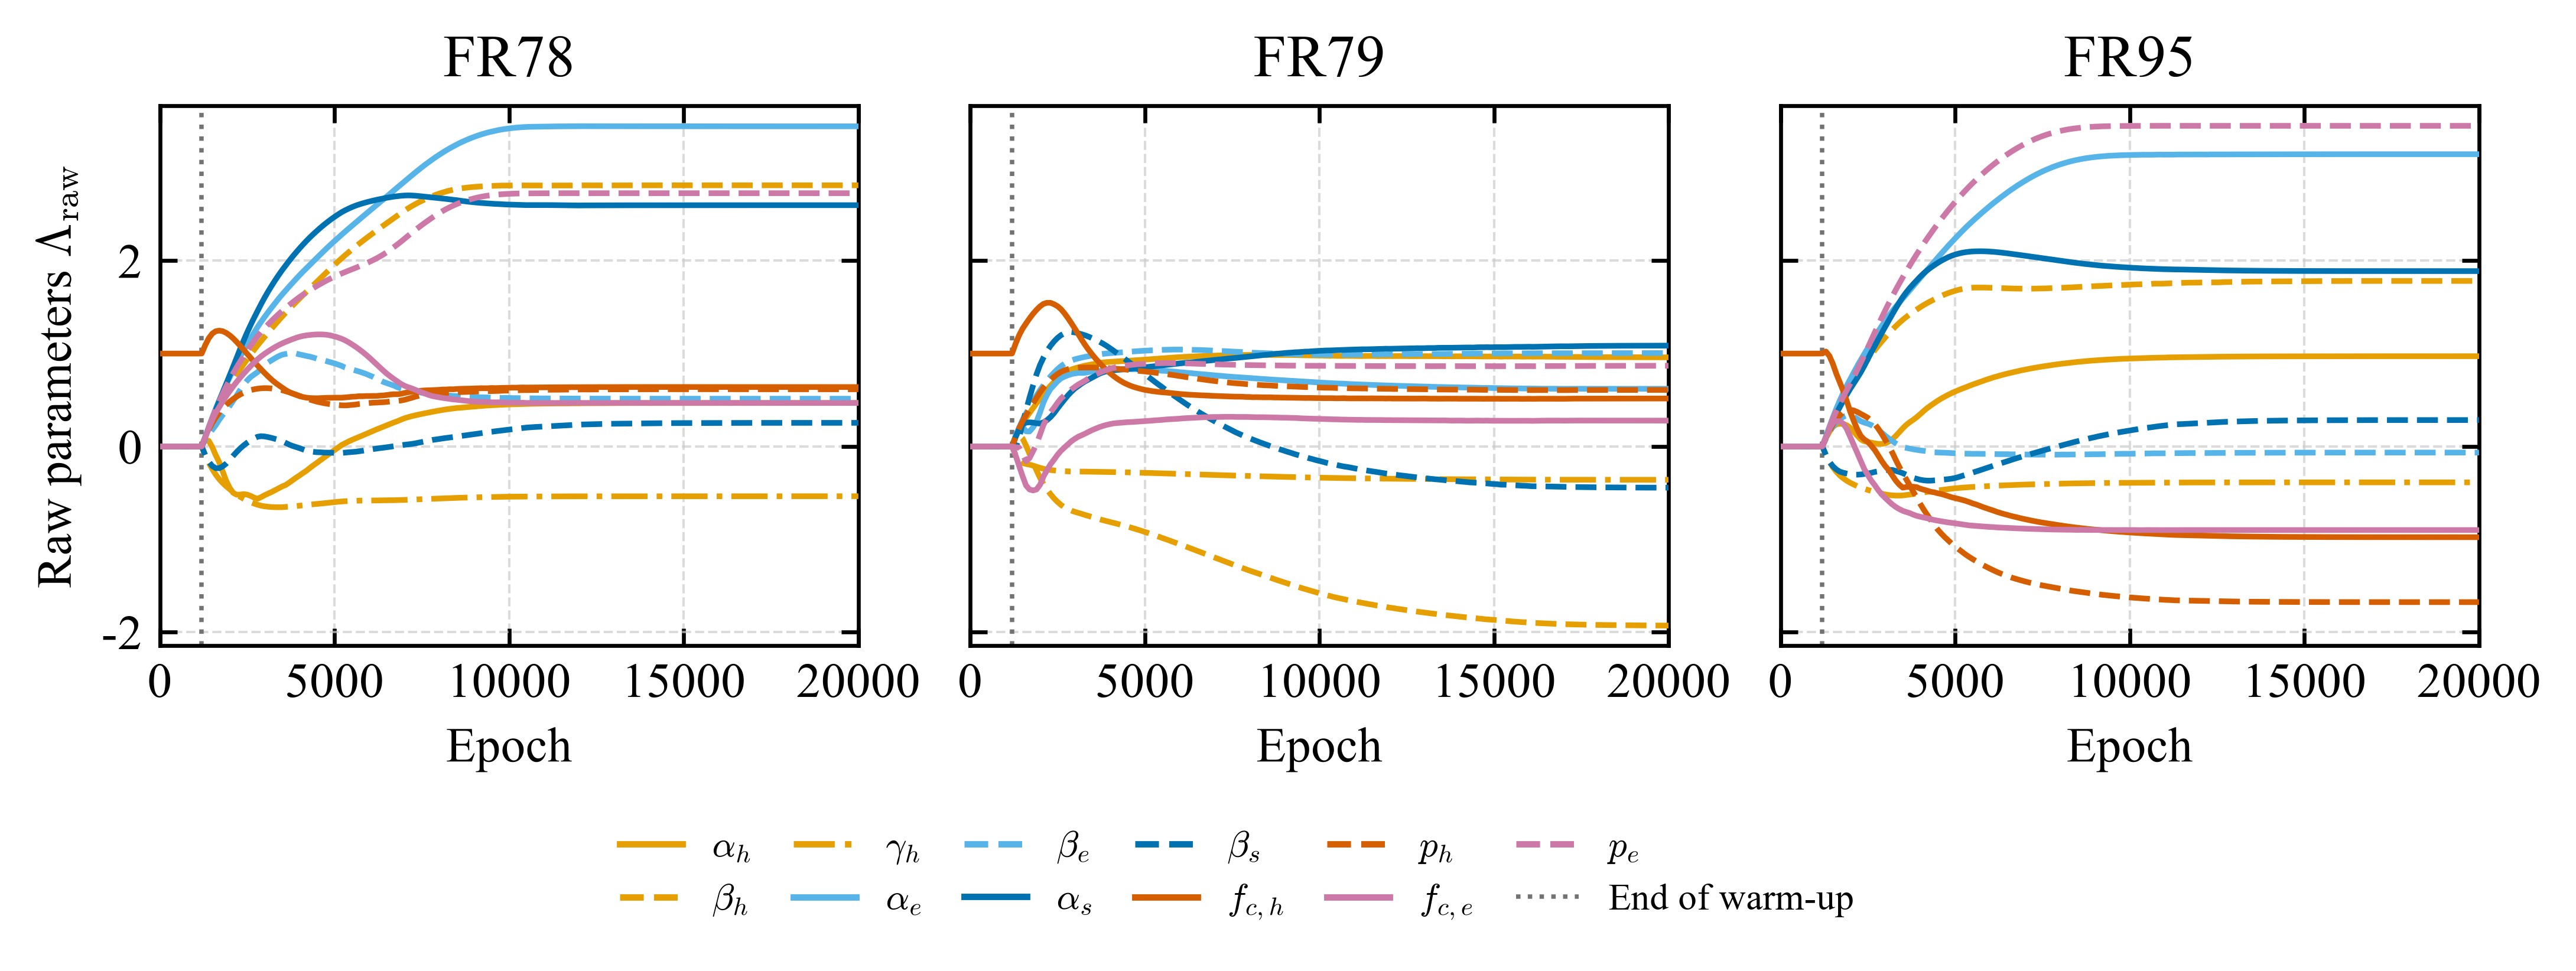
\includegraphics[width=0.98\textwidth]{Figure_parameter_evolution_raw.png}
\caption{Evolution of the raw learnable coordinates for the active LSSI functions. From left to right: FR78, FR79, and FR95. Colors identify mechanism groups and line styles distinguish their parameter components. The anomalous and exponential-saturation coordinates are omitted because their associated candidates are pruned. For clarity, only the first 20,000 epochs are displayed.}
 \label{fig:parameter_evolution}
\end{figure*}

\subsection{Comparison With SE and Fixed-Grid SSI}

For a controlled comparison, every method uses the identical deterministic split. The SE is fitted by linear least squares in logarithmic coordinates. The RF contains 200 trees. The FNN has two 64-neuron hidden layers and 4417 learned weights. SSI uses the 103-term fixed library described in Section~II-B. Table~\ref{tab:comparison} and Fig.~\ref{fig:comparison} report the results. The SE performs reasonably on FR79, where the measured surface is closer to a single power law, but its MAPE rises to $12.76\%$ on FR78 and $10.65\%$ on FR95. The RF improves the two difficult SE cases but is less accurate than the symbolic and neural models. The FNN gives the lowest numerical MAPE for all three materials, between $0.40\%$ and $0.70\%$, confirming the expressive advantage of a black-box mapping. It does not, however, return an explicit equation.

\begin{table*}[t]
\centering
\caption{Held-Out MAPE and Model Complexity Across Materials}
\label{tab:comparison}
\renewcommand{\arraystretch}{1.10}
\begin{tabular}{lccccccl}
\toprule
Method & FR78 (\%) & FR79 (\%) & FR95 (\%) & Learned parameters$^{*}$ & Active terms$^{*}$ & Explicit equation & Model class \\
\midrule
SE   & 12.76 & 2.45 & 10.65 & 3 & 1 & Yes & Fixed empirical \\
RF   & 3.89 & 3.72 & 3.58 & 266732/250886/266732 & -- & No & Black-box ensemble \\
FNN  & \textbf{0.40} & \textbf{0.70} & \textbf{0.49} & 4417 & -- & No & Black-box network \\
SSI  & \textbf{1.90}$^{\dagger}$ & 1.01 & 1.56 & 9/11/7 & 9/11/7 & Yes & Fixed-grid symbolic \\
LSSI & 1.93 & \textbf{0.85}$^{\dagger}$ & \textbf{1.11}$^{\dagger}$ & 15 & \textbf{4} & Yes & Learnable symbolic \\
\bottomrule
\end{tabular}
\vspace{0.5mm}
\footnotesize\raggedright $^{*}$Values separated by slashes correspond to FR78/FR79/FR95. $^{\dagger}$Best evaluated explicit-equation result.
\end{table*}

\begin{figure*}[t]
 \centering
 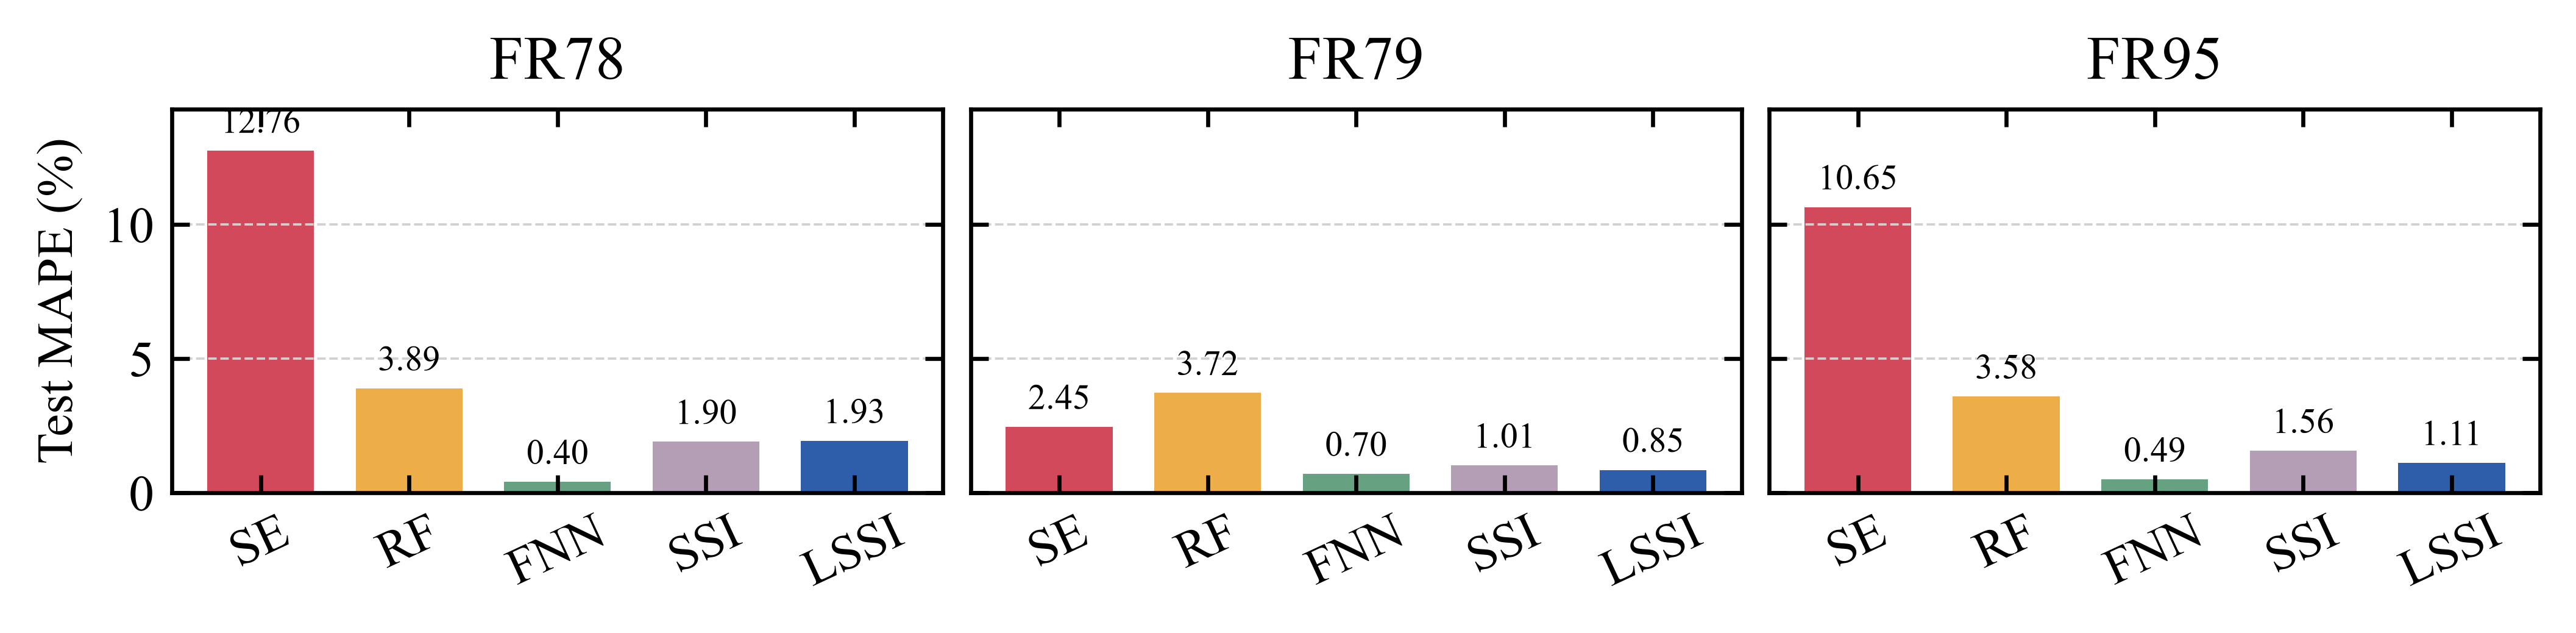
\includegraphics[width=0.98\textwidth]{Figure11_method_comparison.png}
 \caption{Same-split held-out MAPE comparison. From left to right: FR78, FR79, and FR95. The FNN is the most accurate numerical predictor; LSSI gives the lowest three-material mean among the compact explicit equations.}
 \label{fig:comparison}
\end{figure*}

The sparse-model comparison isolates the contribution of learnability. Both SSI and LSSI use physics-motivated terms, nonnegative coefficients, a logarithmic-percentage loss, and thresholded optimization. Their main representational difference is whether internal exponents are fixed or trainable. For FR78, LSSI removes five of nine SSI terms while MAPE increases slightly from $1.90\%$ to $1.93\%$. For FR79, it removes seven of eleven and reduces MAPE by $16\%$ relative; for FR95, it removes three of seven and reduces MAPE by $29\%$. Across all three materials, mean MAPE falls from $1.49\%$ to $1.30\%$. Thus, learnability improves the aggregate accuracy--complexity balance rather than guaranteeing a lower error for every individual surface. Densifying the SSI grid might further reduce its error, but would move in the opposite direction from compactness and introduce still more correlated candidates.

The parameter counts clarify the broader tradeoff. LSSI uses 15 learned quantities in its final four-term equation: four active coefficients and eleven internal parameters belonging to the surviving terms. The FNN obtains lower interpolation error but uses 4417 weights. The RF stores approximately $2.5\times10^5$ learned nodes under the stated 200-tree implementation. These counts do not by themselves prove interpretability, but they show why predictive accuracy and equation discovery must be evaluated as related yet distinct objectives.

Knowledge-aware and physics-informed neural networks represent more advanced predictive baselines \cite{10315145,11126536}. They are not assigned numerical rows in Table~\ref{tab:comparison} because their published results use different datasets, input variables, and validation protocols, and no project implementation is available for retraining on the identical split. Quoting those errors beside the present results would imply a direct comparison that the evidence does not support. The FNN and RF rows are therefore the strongest reproducible black-box comparisons available under controlled data conditions; the cited advanced models define important future benchmarks when same-data implementations become available.

\subsection{Multi-Objective Radar Comparison}

Fig.~\ref{fig:radar} condenses the three material comparisons into one aggregate radar, following the visual convention of the Letter. Accuracy is computed from arithmetic-mean test MAPE across FR78, FR79, and FR95; model complexity uses geometric-mean learned parameter count. Both lower-is-better quantities are inverse min--max mapped to $[1,5]$. The (interpretability, design simplicity, implementation feasibility) triplets are SE $(5,5,5)$, RF $(1.2,2.2,2.5)$, FNN $(1,3,3)$, SSI $(4.6,4.5,4.8)$, and LSSI $(5,4.8,5)$; overall benefit is the five-axis mean. Thus, only one envelope is drawn per method.

\begin{figure}[t]
 \centering
 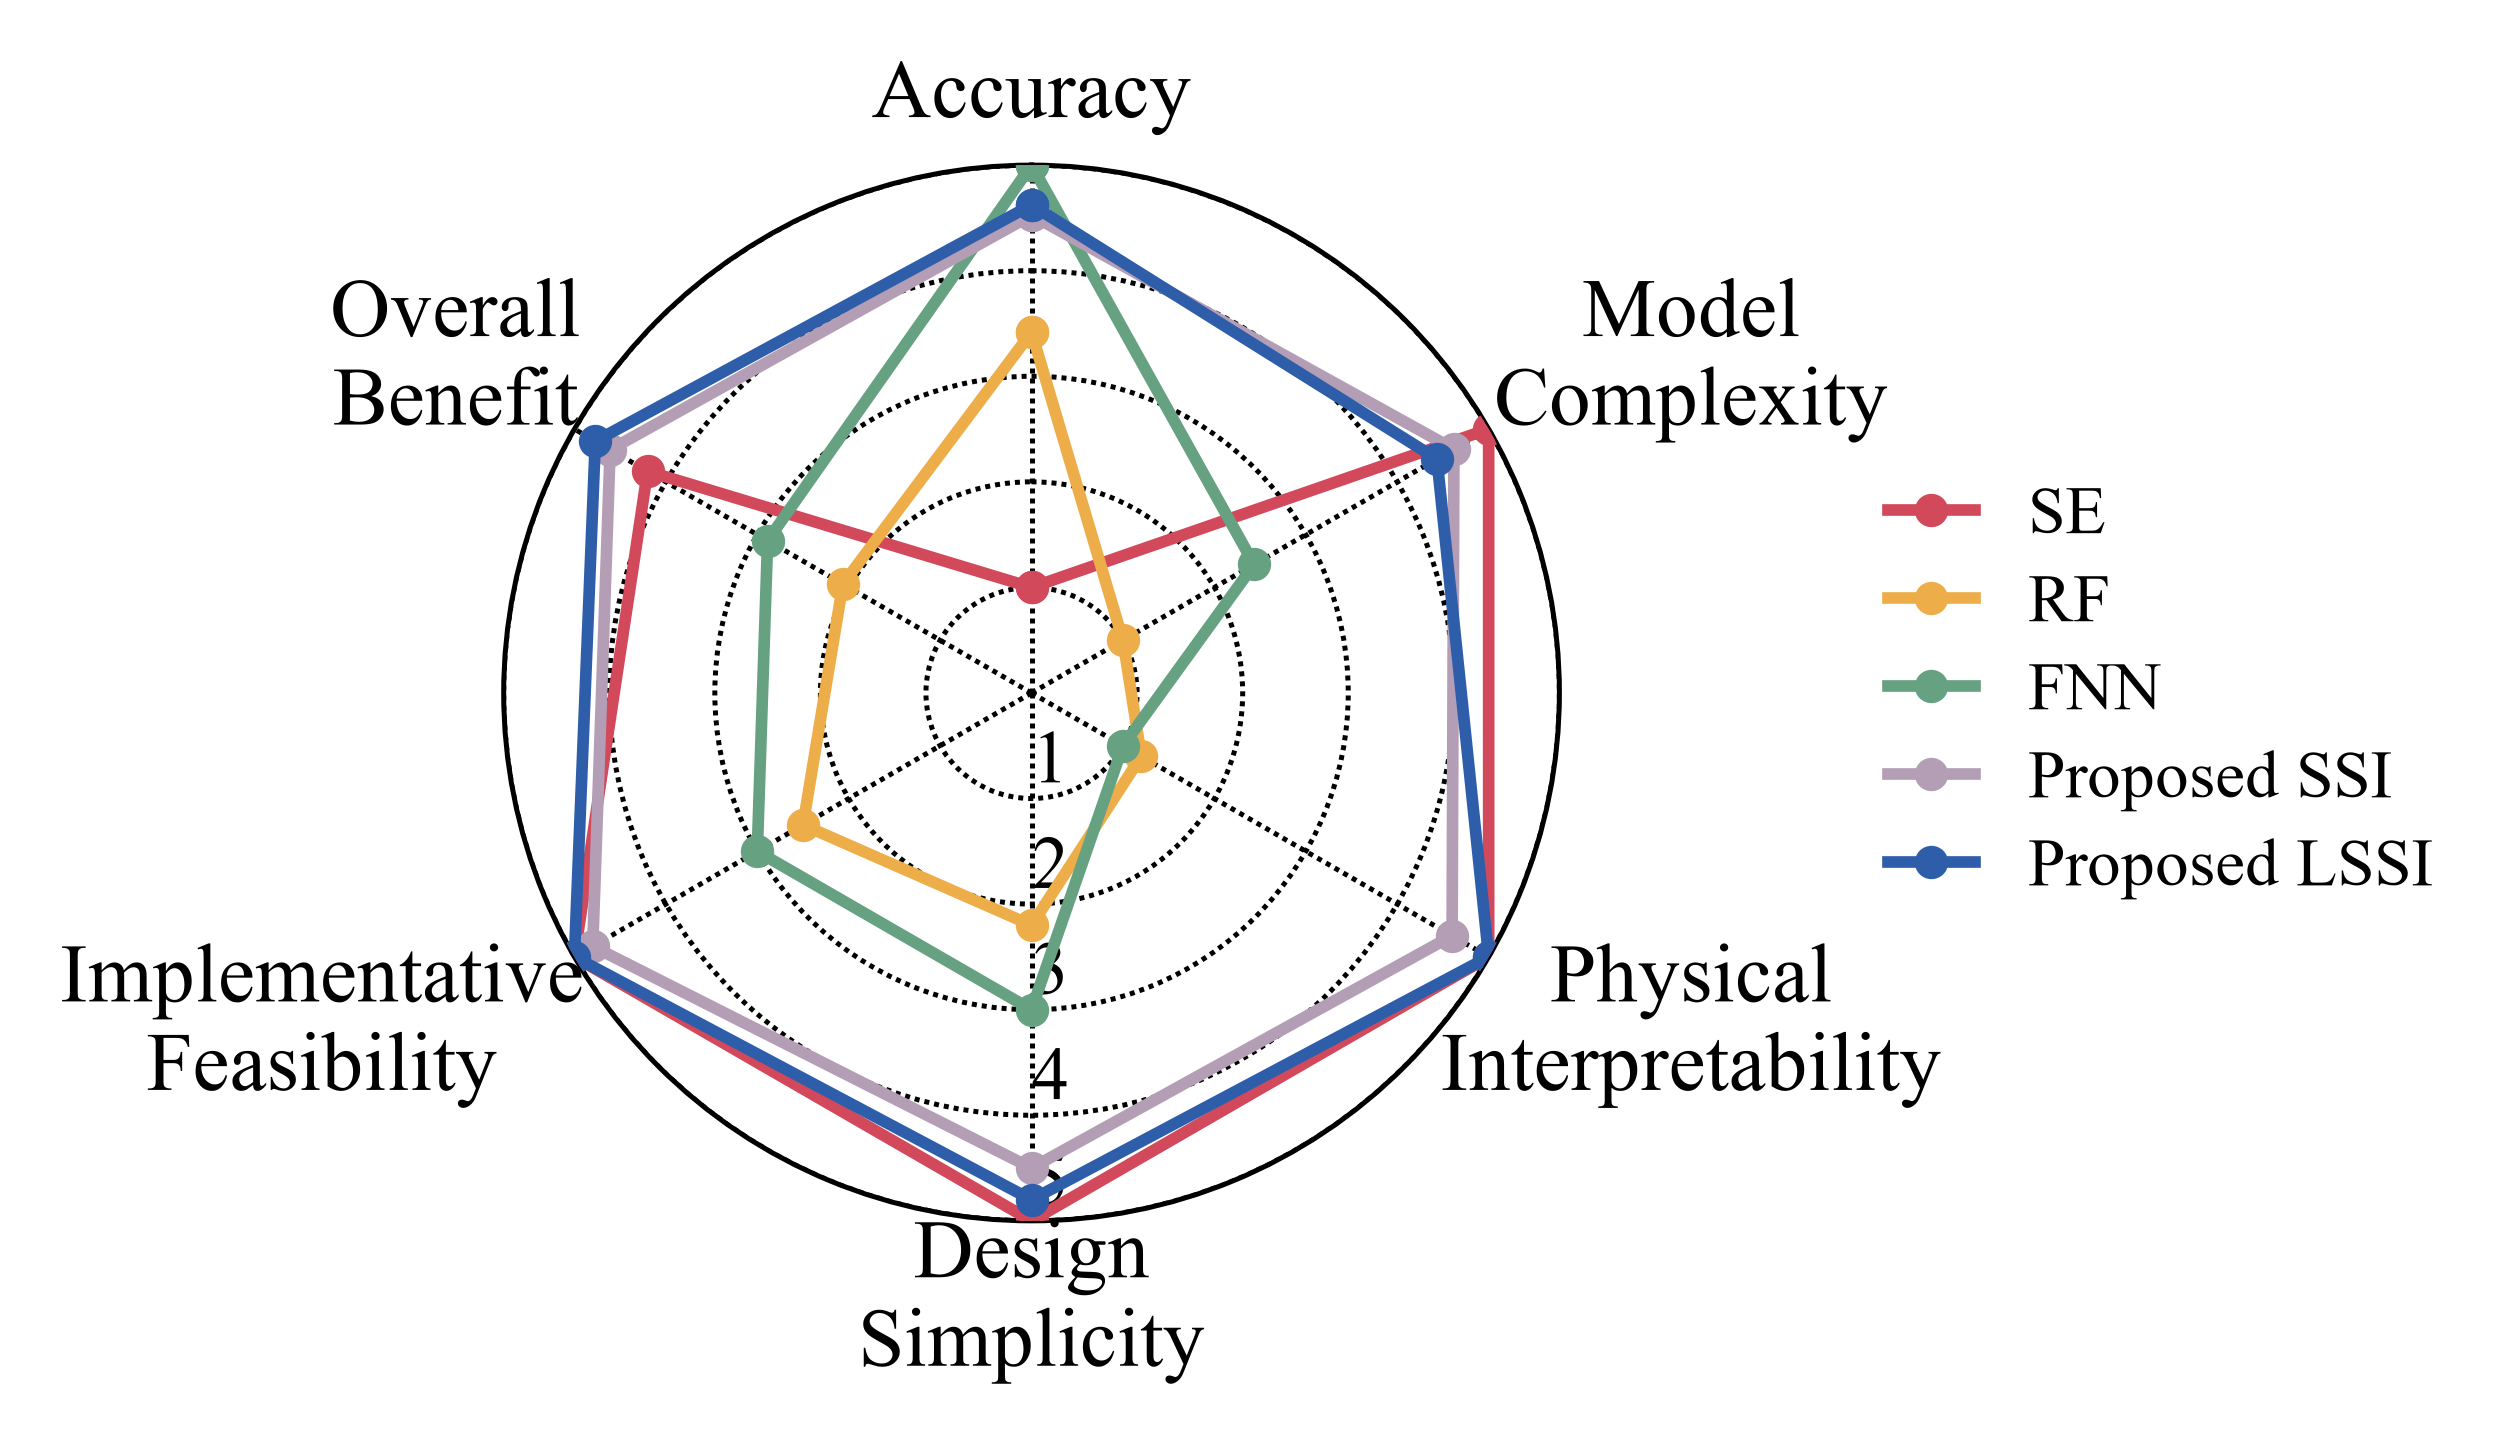
\includegraphics[width=0.98\columnwidth]{Figure12_combined_radar.png}
 \caption{Single aggregate multi-objective comparison across FR78, FR79, and FR95. LSSI provides the most balanced envelope, whereas the FNN leads pure prediction accuracy and the SE leads parameter compactness.}
 \label{fig:radar}
\end{figure}

On the aggregated accuracy axis, the FNN leads because its mean test MAPE is $0.53\%$, followed by LSSI at $1.30\%$ and SSI at $1.49\%$. The SE is maximally compact but has a mean MAPE of $8.62\%$. SSI remains explicit, yet its 7--11 fixed-grid terms reduce design simplicity. LSSI stays near the outer boundary on five axes and remains competitive on accuracy. The radar result therefore supports the intended claim: LSSI is not an attempt to make a four-term equation numerically outperform every unrestricted black box; it moves the accuracy--interpretability Pareto frontier of explicit core-loss equations.

\subsection{Late-Stage Convergence Audit}

Convergence is evaluated with one common rule rather than by visual judgment. The state at epoch 31,200, which corresponds to 75\% of joint discovery after the 1200-epoch warm-up, is compared with the final AdamW state at epoch 41,100. The maximum absolute changes in any sparse coefficient are $7.81\times10^{-5}$, $1.20\times10^{-4}$, and $1.01\times10^{-4}$ for FR78, FR79, and FR95. The corresponding maxima over the eleven active raw coordinates are $7.88\times10^{-4}$, $8.95\times10^{-4}$, and $7.02\times10^{-4}$. All are below the shared tolerances of $1.5\times10^{-4}$ and $10^{-3}$, respectively. This audit is especially important for FR79: extending the original unregularized run alone preserved coefficient exchange, whereas the common weak regularizer removes that flat direction without changing its four-term support.

\section{Physical Interpretation and Design Implications}
\subsection{A Shared Structure With Material-Specific Parameters}

The identified coefficients and parameters in Table~\ref{tab:identified} separate topology from parameterization. The same four candidates survive for all materials, yet their relative contributions and exponents change. The hysteresis-like term contributes approximately 34--38\% in every case. This consistency supports its role as a base mechanism across the tested operating regions. The eddy-current-like share is about 30\% for FR78 and 35\% for FR95, but only 9\% for FR79. Conversely, the steep saturation correction contributes 55\% for FR79, compared with 30\% for FR78 and 25\% for FR95. FR79 therefore cannot be summarized as merely a rescaled FR95 equation; it requires a different balance among the same mechanisms.

\begin{figure*}[t]
 \centering
 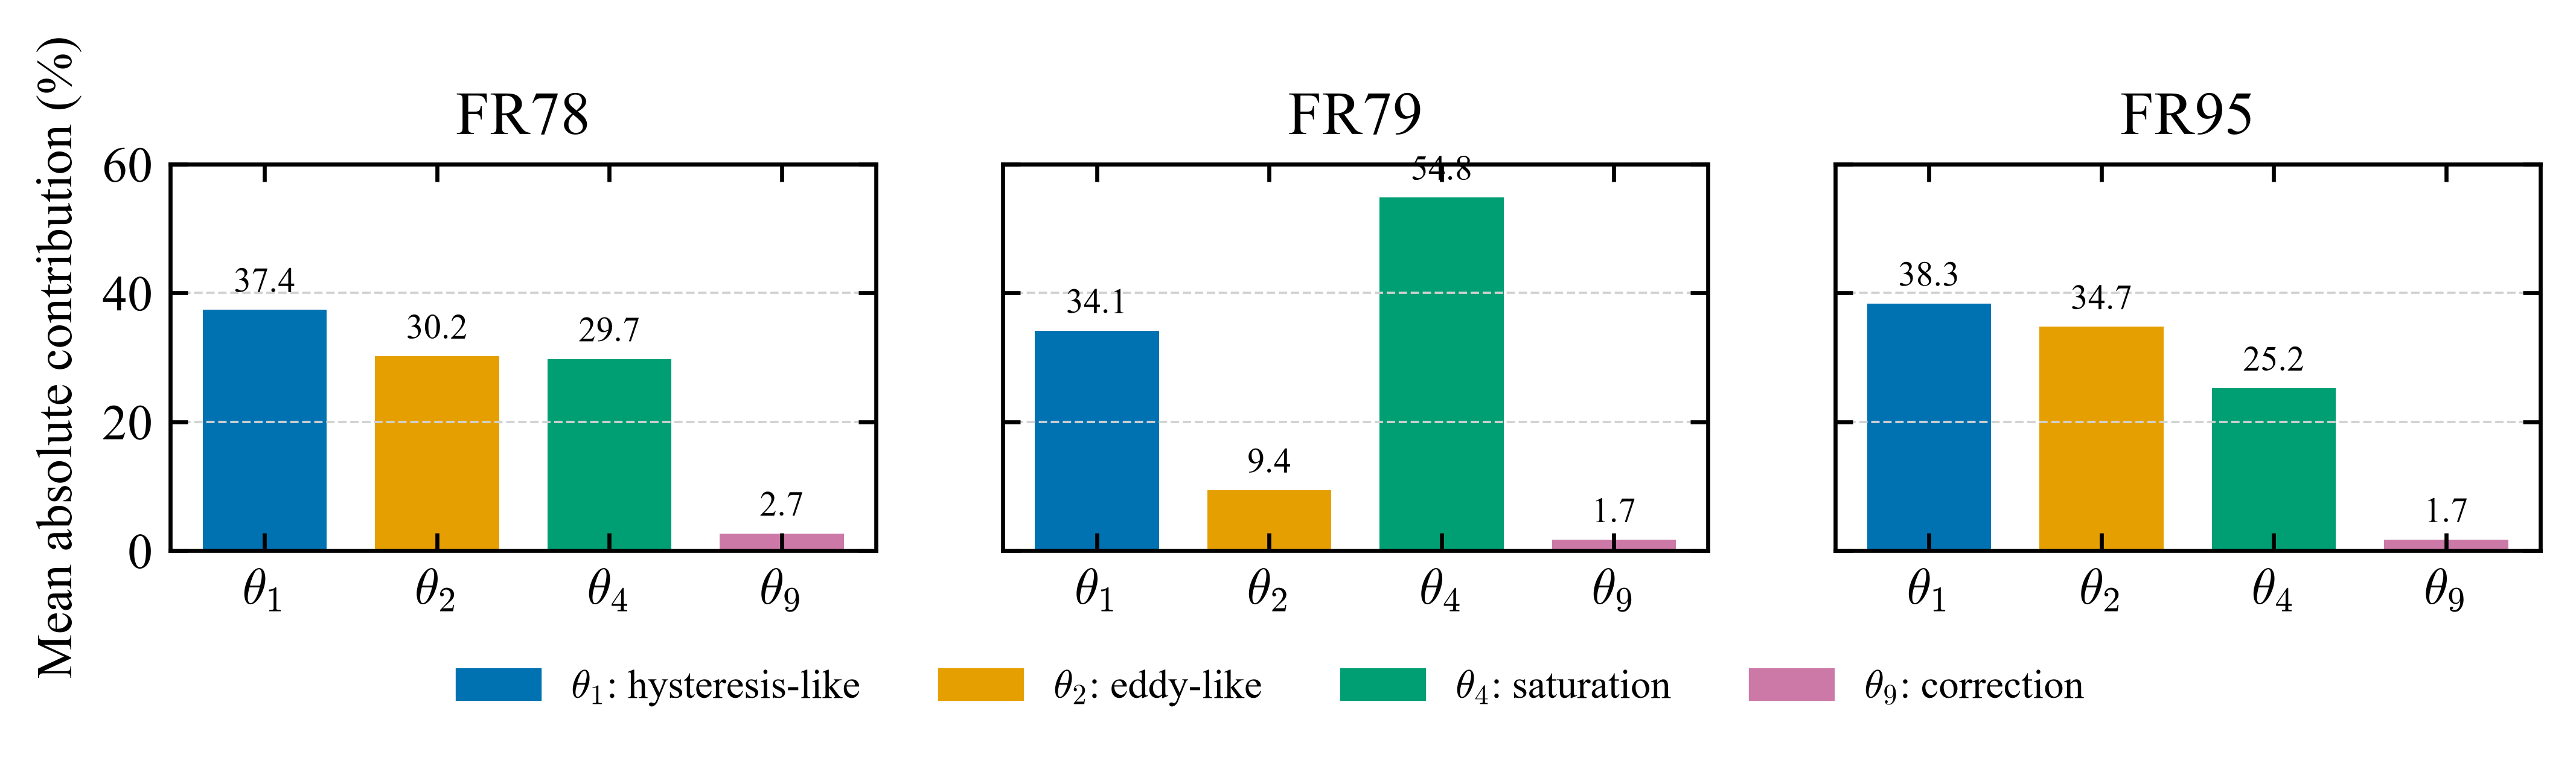
\includegraphics[width=0.94\textwidth]{Figure13_common_structure.png}
 \caption{Mean absolute contributions of the four retained LSSI terms. From left to right: FR78, FR79, and FR95. The identical four-term support establishes the common topology, while the contribution changes quantify material-specific mechanism balance.}
 \label{fig:common_structure}
\end{figure*}

The learned eddy-current exponents remain close to the classical pair $(2,2)$: $\alpha_e$ lies between 2.060 and 2.188 and $\beta_e$ between 1.993 and 2.093. The saturation flux exponents are consistently larger, between 3.073 and 3.200. Hysteresis-like frequency exponents remain near unity, whereas $\beta_h$ varies more strongly from 2.101 for FR79 to 2.755 for FR78. These ranges are physically legible in a way that a list of neighboring fixed-grid terms is not.

The negative $\gamma_h$ values mean that the local flux exponent of Candidate 1 decreases as normalized flux rises. Candidate 4 simultaneously supplies a steep high-flux contribution. Together these two functions allow the effective slope of total loss to change across the domain without summing many closely spaced powers. The small $\xi_9\Bbar$ correction contributes only 1.68--2.68\% but consistently reduces low-loss bias. Because its contribution is above the common $0.1\%$ cutoff for all three materials, it is retained rather than dismissed as numerical noise.

The cutoff parameters also reveal where dispersion becomes important. For FR95, the Candidate-2 cutoff is approximately \SI{1176}{\kilo\hertz}, near the upper edge of the measured band, whereas the Candidate-1 cutoff is approximately \SI{1830}{\kilo\hertz}. The FR78 and FR79 hysteresis-like cutoffs are approximately \SI{2.9}{\mega\hertz} and \SI{2.7}{\mega\hertz}, respectively, so $R_h$ stays close to unity over most sampled points. These values should be interpreted as effective macroscopic scales, not direct microscopic relaxation frequencies, especially when an estimated cutoff lies outside the measurement envelope.

\subsection{Use in Magnetic Design}

The final equation is differentiable and inexpensive. For a candidate core volume $V_c$, the core dissipation under sinusoidal excitation is simply $P_{\mathrm{core}}=V_cP_{\mathrm{n}}\Pbar$. Its local logarithmic sensitivities,
\begin{equation}
 S_f=\frac{\partial\ln P_v}{\partial\ln f},\qquad
 S_B=\frac{\partial\ln P_v}{\partial\ln B},
 \label{eq:sensitivity}
\end{equation}
can be evaluated analytically or by automatic differentiation. Unlike the constant SE exponents, $S_f$ and $S_B$ vary with operating point because the relative contribution of each term and the roll-off factors change. This gives a designer a direct answer to whether reducing flux density or switching frequency is more effective at the current operating point.

The compact form is also suitable for loss-constrained optimization. If winding geometry relates $B$ to turns, voltage, and frequency, (\ref{eq:identified}) can be embedded directly in a continuous optimizer without calling a tree ensemble or network runtime. The nonnegative decomposition supports diagnostic plots: term contributions show whether an operating point is dominated by the base hysteresis-like component, the eddy-current-like component, or the high-flux correction. Such information can guide material selection and determine where new measurements would most reduce uncertainty.

The method is not intended to replace physics with arbitrary regression. Its value is to place physical hypotheses in a testable library and let data determine their support and continuous scaling. If a candidate repeatedly prunes across materials, it is empirically unnecessary for the stated domain. If it survives with a stable exponent, it becomes a concise hypothesis that can be compared with material theory and additional experiments.

\section{Scope, Limitations, and Extensions}

The validation covers sinusoidal excitation at \SI{25}{\degreeCelsius} and interpolation inside the measured $f$--$B$ envelope. Nonsinusoidal waveforms, dc bias, temperature, and extrapolation require additional inputs and data; future tests should reserve contiguous boundary regions and quantify uncertainty. Temperature-dependent coefficients and waveform descriptors can extend LSSI without changing the separation between topology selection and continuous parameter adaptation. A parameter repeatedly reaching its bound would instead indicate that the library or bounds require revision.

The retained terms are mechanism-inspired but inferred from aggregate loss. Because similar finite-domain scaling can prevent a unique microscopic decomposition, Fig.~\ref{fig:common_structure} is an effective design-oriented attribution; complex-permeability, domain-dynamic, or temperature-dependent measurements are needed for stronger physical identification.

\section{Conclusion}

LSSI replaces a large fixed symbolic grid with ten physics-guided functions whose fractional exponents and roll-off parameters are learned jointly with nonnegative sparse coefficients. Across 3880 FR78, FR79, and FR95 measurements, it recovered the same four-term support and achieved held-out MAPEs of $1.93/0.85/1.11\%$ with $R^2\geq0.9995$. Relative to 103-term fixed-grid SSI, the final equation shrank from 7--11 terms to four while reducing mean MAPE from $1.49\%$ to $1.30\%$; FR78 exposes the honest tradeoff that maximal compression need not improve every individual dataset.

The cross-material evidence yields three conclusions: a hysteresis-like, eddy-current-like, high-flux, and low-order correction topology transfers across the ferrites; continuous parameter learning is more efficient than combining neighboring fixed powers; and FNNs reduce interpolation error only by sacrificing the explicit equation. LSSI therefore advances the accuracy--interpretability frontier and retains analytical sensitivities suitable for magnetic characterization and converter optimization.

\bibliographystyle{IEEEtran}
\bibliography{Bibliography/references}

\end{document}
